\documentclass[../main.tex]{subfiles}



\begin{document}
\section{Mechanika klasyczna}
\textit{I have not been able to discover the cause of those properties of gravity from phenomena,
and I frame no hypotheses; for whatever is not deduced from the phenomena is to be called a
hypothesis, and hypotheses, whether metaphysical or physical, whether of occult qualities or
mechanical, have no place in experimental philosophy.}\begin{flushright}Sir Isaac
Newton\end{flushright}

\begin{table}[h]
    \centering
    \begin{tabular}{ *5l }\toprule \emph{Jednostka} & \emph{Symbol} & \emph{Wielkość fizyczna}
    \\\midrule metr    & m  & długość   \\ 
    sekunda  & s & czas  \\ 
    kilogram  & kg & masa  \\
    mol     & mol  & liczność materii   \\ 
    amper  & A & natężenie prądu elektrycznego\\ 
    kelwin & K & temperatura termodynamiczna  \\
    kandela & cd & światłość\\
    \bottomrule
    \hline
\end{tabular}
\caption{Jednostki podstawowe układu SI}
\end{table}
\subsection{Przestrzeń i czas}
Podstawową rolę w opisywaniu jakichkolwiek zjawisk fizycznych pełnią dwa parametry: wektor wodzący
\(\mathbf{r}\) wyznaczający położenie danego punktu w przestrzeni oraz czas \(t\). W mechanice
klasycznej (za Newtonem) przyjmujemy, że czas jest globalnym, uniwersalnym parametrem, który zmienia
się jednakowo dla wszystkich obserwatorów.
\subsubsection{Podstawowe działania na wektorach}
Niech dane będą dwa wektory \(\mathbf{a}=[a_1,a_2,a_3]\) i \(\mathbf{b}=[b_1,b_2,b_3]\).

\begin{itemize}
    \item dodawanie wektorów
    \begin{equation*}
        \mathbf{a}\pm\mathbf{b}=[a_1\pm b_1, a_2\pm b_2,a_3\pm b_3 ]
    \end{equation*}
    
    \item mnożenie wektora przez skalar
    \begin{equation*}
        k\mathbf{a}=[ka_1,ka_2,ka_3]
    \end{equation*}
    \item iloczyn wektorowy
    \begin{equation*}
    \begin{split}
       \mathbf{a}\times\mathbf{b}=[a_2b_3-a_3b_2,a_3b_1-a_1b_3,a_1b_2-a_2b_1]
    \end{split}
    \end{equation*}
    
    \item iloczyn skalarny
    \begin{equation*}
        \mathbf{a}\cdot\mathbf{b}=a_1b_1+a_2b_2+a_3b_3
    \end{equation*}
    \item różniczkowanie wektorów
    \begin{equation*}
        \dot{\mathbf{a}}=\dv{\mathbf{a}}{t}=\sum_{\alpha=1}^3\left(\dot a_\alpha\mathbf{\hat e}_\alpha+a_\alpha\dv{\mathbf{\hat e_\alpha}}{t}\right)
    \end{equation*}
    We współrzędnych kartezjańskich \((\mathbf{\hat e}_1,\mathbf{\hat e}_2,\mathbf{\hat
    e}_3)=(\mathbf{\hat x},\mathbf{\hat y},\mathbf{\hat z})\)
    \begin{equation*}
        \dot{\mathbf{a}}=\dot a_x\mathbf{\hat x}+\dot a_y\mathbf{\hat y}+\dot a_z\mathbf{\hat z}
    \end{equation*}
\end{itemize}
\subsubsection{Zasady dynamiki Newtona}
\begin{enumerate}[I.]
    \item Istnieją takie układy odniesienia (nazywane układami inercjalnymi), w których gdy siła
    wypadkowa działająca na ciało wynosi zero to ciało pozostaje w spoczynku lub porusza się ruchem
    jednostajnym prostoliniowym.
    \item W inercjalnych układach odniesienia siła wypadkowa działająca na ciało jest równa
    pierwszej pochodnej pędu tego ciała po czasie.
    \begin{equation*}
        \mathbf{F}=\dot{\mathbf{p}}\,.
    \end{equation*}
    \item Jeżeli ciało A działa na ciało B siłą o wartości \(F\) to również ciało B działa na ciało
    A siłą o takiej samej wartości, tym samym kierunku, ale przeciwnym zwrocie.
\end{enumerate}
\newpage
\subsection{Ruch pocisków}
Następne rozważania będą dotyczyć punktów materialnych. \textit{Punktem materialnym nazywamy ciało
obdarzone masą, którego objętość możemy pominąć.} Jeżeli masa ciała \(m\) jest stała oraz siła
wypadkowa działająca na nie nie jest funkcją czasu \(\dot{\mathbf{F}}=0\), wówczas korzystając z II
zasady dynamiki łatwo możemy znaleźć równanie ruchu tego ciała, tj. funkcję \(\mathbf{r}(t)\). W
układzie współrzędnych kartezjańskich mamy
\begin{equation*}
    \mathbf{F}=[F_x,F_y,F_z]=m[\ddot x,\ddot y, \ddot z]\,,
\end{equation*}
skąd przez całkowanie otrzymujemy
\begin{equation*}
    \begin{split}
    &x(t)=\frac{F_x}{2m}t^2+v_x(0)t+x(0)\\
    &y(t)=\frac{F_y}{2m}t^2+v_y(0)t+y(0)\\
    &z(t)=\frac{F_z}{2m}t^2+v_z(0)t+z(0)\,.
    \end{split}
\end{equation*}
\subsubsection{Rzut ukośny z pominięciem oporów powietrza}
Zajmiemy się teraz problemem rzutu ukośnego w jednorodnym polu grawitacyjnym, w którym na ciało
działa jedynie siła ciężkości \(\mathbf{F}=-mg\mathbf{\hat y}\). Problem ten jest w istocie
problemem dwuwymiarowym, więc przyjmując kartezjański układ współrzędnych z osią \(y\) zwróconą w
górę i korzystając z poprzednich wyników mamy
\begin{equation*}
\begin{split}
    &x(t)=v_x(0)t+x(0)\\
    &y(t)=-\frac{1}{2}gt^2+v_y(0)+y(0)\,.
\end{split}
\end{equation*}
Przyjmijmy następujące, ogólne warunki początkowe: ciało znajduje się początkowo w punkcie \(x=0\),
\(y=h_0\), prędkość początkowa ciała ma wartość \(v_0\), wektor prędkości początkowej jest nachylony
pod kątem \(\theta\) do poziomu. Wówczas mamy
\begin{equation*}
    \begin{split}
        &x(t)=v_0\cos\theta\,t\\
        &y(t)=-\frac{1}{2}gt^2+v_0\sin\theta\,t+h_0\,.
    \end{split}
\end{equation*}
Wyznaczając z pierwszego równania \(t\) i podstawiając do drugiego równania otrzymujemy równanie
trajektorii pocisku \(y(x)\)
\begin{equation*}
    y(x)=h_0+x\tan\theta-\frac{g}{2v_0^2\cos^2\theta}\,x^2\,.
\end{equation*}
Zasięg rzutu \(Z\) możemy znaleźć  rozwiązując równanie kwadratowe \(y(Z)=0\)
\begin{equation*}
    Z=v_0\cos\theta\frac{v_0\sin\theta+\sqrt{v_0^2\sin^2\theta+2gh_0}}{g}\,,
\end{equation*}
dla \(h_0=0\) otrzymujemy znajomą postać \(Z=\frac{v_0^2}{g}\sin2\theta\). Kąt
\(\theta_\text{max}\), dla którego zasięg jest maksymalny obliczamy rozwiązując równanie
\(\frac{dZ(\theta)}{d\theta}|_{\theta_\text{max}}=0\), skąd otrzymujemy
\begin{equation*}
    \cos\theta_\text{max}=\frac{\sqrt{2gh_0+v_0^2}}{\sqrt{2gh_0+2v_0^2}}\,,
\end{equation*}
dla \(h_0=0\) otrzymujemy oczywiście \(\theta_\text{max}=45^\circ\).
\subsubsection*{Trafienie w linię zbocza}
Rozpatrzmy następujący problem: armata ustawiona na wysokości \(h_0=0\) wystrzeliwuje pociski z
prędkością początkową \(v_0\) pod dowolnym kątem z zakresu \((0^\circ,90^\circ)\). Znaleźć
współrzędne punktu trafienia \((x_1,y_1)\) w linię zbocza daną równaniem \(Y(x)=(x-x_0)\tan\beta\).
Równanie toru pocisku ma postać
\begin{equation*}
    y(x)=x\tan\theta-\frac{g}{2v_0^2\cos^2\theta}\,x^2\,.
\end{equation*}
Współrzędne punktu trafienia muszą spełniać oba równania, tj. \(y(x_1)=Y(x_1)=y_1\). Mamy zatem
\begin{equation*}
\begin{split}
    \frac{gx_1^2}{2v_0^2\cos^2\theta}+x_1(\tan\beta-\tan\theta)-x_0\tan\beta=0
\end{split}
\end{equation*}
oraz
\begin{equation*}
    y_1=(x_1-x_0)\tan\beta\,.
\end{equation*}
Rozwiązując równanie kwadratowe otrzymujemy
\begin{equation*}
\begin{split}
    x_1=\frac{v_0^2\cos^2\theta}{g}\Bigg(\tan\theta-\tan\beta+\sqrt{(\tan\beta-\tan\theta)^2+\frac{2gx_0\tan\beta}{v_0^2\cos^2\theta}}\,\Bigg)\,.
\end{split}
\end{equation*}
\subsubsection*{Obwiednia trajektorii pocisków}
Rozpatrzmy następujący problem: fontanna jest zbudowana z punktowego źródła znajdującego się w
początku układu współrzędnych, wystrzeliwującego wodę z jednakową prędkością \(v_0\) we wszystkich
kierunkach \((0^\circ;180^\circ)\). Należy znaleźć kształt fontanny. Równanie trajektorii fragmentu
wody wystrzelonego pod katem \(\theta\) ma postać
\begin{equation*}
    y(x)=x\tan\theta-\frac{g}{2v_0^2\cos^2\theta}\,x^2\,.
\end{equation*}
Rozpatrzmy punkt o współrzędnych \((x_\alpha,y_\alpha)\). Aby sprawdzić, czy możliwe jest aby
fragment wody trafił w ten punkt należy rozwiązać równanie
\begin{equation*}
    y_\alpha=x_\alpha\tan\theta-\frac{g}{2v_0^2\cos^2\theta}\,x_\alpha^2\,.
\end{equation*}
względem \(\theta\). Korzystając z tożsamości \(\sec^2\theta=1+\tan^2\theta\) i podstawiając
\(u=\tan \theta\) możemy przepisać to równanie do postaci
\begin{equation*}
    \frac{gx_\alpha^2}{2v_0^2}\,u^2-x_\alpha u+\left(y_\alpha+\frac{g}{2v_0^2}\right)=0\,.
\end{equation*}
Jest to równanie kwadratowe zmiennej \(u\). Równanie to posiada rozwiązania rzeczywiste wtedy i
tylko wtedy gdy \(\Delta \geq0\), zatem
\begin{equation*}
    \begin{split}
        \Delta = &x_\alpha^2-\frac{4gx_\alpha^2}{2v_0^2}\left(y_\alpha+\frac{g}{2v_0^2}\right)\geq0\\
        &y_\alpha\leq \frac{v_0^2}{2g}-\frac{gx_\alpha^2}{2v_0^2}\,.
    \end{split}
\end{equation*}
Ostatnia nierówność wyznacza obszar, w którym znajdują się punkty o współrzędnych
\(x_\alpha,y_\alpha\), do których trafiają fragmenty wody. Konturem tego obszaru jest parabola
\begin{equation*}
   y(x)=\frac{v_0^2}{2g}-\frac{gx^2}{2v_0^2}\,.
\end{equation*}
Jest to zarówno szukany kształt fontanny oraz obwiednia trajektorii pocisków wystrzelonych z
jednakowymi szybkościami.
\medskip

Obwiednię trajektorii pocisków możemy również znaleźć tak jak w kursach analizy matematycznej.
Istotnie jeśli zapiszemy trajektorię pocisku jako
\begin{equation*}
    F(u,x,y)=f_u(x,y)=0\,,
\end{equation*}
gdzie \(u\) jest pewnym parametrem (np. kątem wystrzału) to obwiednią wszystkich trajektorii będzie
zbiór punktów \(E\)
\begin{equation*}
    E=\left\{(x,y):f_u(x,y)=0\quad\land\quad \pdv{F}{u}=0\right\}\,.
\end{equation*}
Dla naszego problemu mamy
\begin{equation*}
    F(\theta,x,y)=x\tan\theta-\frac{gx^2}{2v_0^2\cos^2\theta}-y=0\,,
\end{equation*}
skąd otrzymujemy warunek
\begin{equation*}
    \partial_\theta F=\sec^2\theta\left(x-\frac{gx^2}{v_0^2}\tan\theta\right)=0\,.
\end{equation*}
Z powyższego zatem \(\tan\theta=v_0^2/gx\) i \(\sec^2\theta=1+v_0^4/g^2x^2\), skąd
\begin{equation*}
    E=\left\{(x,y): y=\frac{v_0^2}{2g}-\frac{gx^2}{2v_0}\right\}\,.
\end{equation*}
\medskip

{\textbf{\textit{Zadanie.}}}
\textit{W wierzchołkach \(n\)-kąta foremnego znajdują się pociski balistyczne. Pocisku w wierzchołku \(k\) jest ciągle naprowadzany na pocisk w wierzchołku \(k+1\) tak, że pociski gonią się nawzajem. Bok wielokąta ma długość \(l\), natomiast szybkość każdego pocisku wynosi \(v\). Wyznacz drogę \(s\) jaką przebędzie każdy z pocisków do chwili spotkania.}
\medskip

\textit{Rozwiązanie. \medskip}

Niech \(t\) oznacza czas po jakim pociski się spotkają. Droga jaką każdy pocisk przebędzie do
spotkania wynosi po prostu \(s=vt\). Prędkość względna wzdłuż boku łączącego dwa kolejne pociski
wynosi \(v_\text{wzg}=v-v\sin\left(\theta-\frac{\pi}{2}\right)\), gdzie \(\theta=\pi\frac{n-2}{2}\)
jest kątem wewnętrznym \(n\)-kąta foremnego. Czas \(t\) wynosi zatem \(t=\frac{l}{v_\text{wzg}}\), a
zatem
\begin{equation*}
    s=vt=\frac{vl}{v_\text{wzg}}=\frac{l}{1+\cos\left(\pi\frac{n-2}{n}\right)}\,.
\end{equation*}
\subsubsection{Opór powietrza}
Siłę oporu powietrza możemy w ogólny sposób zapisać jako \(\mathbf{F}_\text{op}=-f(v)\mathbf{\hat
v}\), gdzie \(v\) jest szybkością ciała. Dla niewielkich szybkości możemy skorzystać ze wzoru
Taylora i przybliżyć funkcję \(f\): \(f(v)=bv+cv^2\) (czynimy tu założenie, że dla zerowej szybkości
siła oporu również jest zerowa). Człon liniowy \(bv\) opisuje opór lepki, na ogół proporcjonalny do
lepkości ośrodka i rozmiarów pocisku.
\subsubsection*{Liniowy opór powietrza}
Zajmiemy się analizą ruchu pocisku poddanego działaniu siły ciężkości \(-mg\mathbf{\hat y}\) i
liniowej siły oporu \(-b\mathbf{v}\). Korzystając z drugiej zasady dynamiki mamy
\begin{equation*}
    m[\ddot x,\ddot y]=-mg[0,1]-b[\dot x,\dot y]\,.
\end{equation*}
Otrzymujemy więc dwa niezależne równania różniczkowe:
\begin{equation*}
    \begin{split}
        &\ddot x=-\frac{b}{m}\dot x\\
        &\ddot y=-g-\frac{b}{m}\dot y\,,
    \end{split}
\end{equation*}
które możemy łatwo rozwiązać przez separację zmiennych i całkowanie  
\begin{equation*}
    \begin{split}
        &\int\frac{\dd\dot x}{\dot x}=-\frac{b}{m}\,\int \dd t\\
        &\int\frac{\dd\dot y}{g+\frac{b}{m}\dot y}=-\int \dd t
    \end{split}
\end{equation*}
\begin{equation*}
    \begin{split}
        &\ln\dot x+C_1=-\frac{b}{m}t\\
        &\frac{m}{b}\ln\left|g+\frac{b}{m}\dot y\right|+C_2=-t\,,
    \end{split}
\end{equation*}
gdzie \(C_1\), \(C_2\) to stałe całkowania równe odpowiednio \(C_1=-\ln\dot x(0)\) oraz
\(C_2=-\frac{m}{b}\ln|g+\frac{b}{m}\dot y(0)|\).
\begin{equation*}
\begin{split}
    &\ln\left(\frac{\dot x}{\dot x(0)}\right)=-\frac{b}{m}t\\
    &\ln\left(\frac{g+\frac{b}{m}\dot y}{g+\frac{b}{m}\dot y(0)}\right)=-\frac{b}{m}t\,,
\end{split}
\end{equation*}
skąd ostatecznie
\begin{equation*}
    \begin{split}
        &\dot x(t)=\dot x(0)e^{-\frac{b}{m}t}\\
        &\dot y(t)=-\frac{mg}{b}\left(1-e^{-\frac{b}{m}t}\right)+\dot y(0)e^{-\frac{b}{m}t}\,.
    \end{split}
\end{equation*}
\subsubsection*{Rzut ukośny z liniowym oporem powietrza}
Całkując wyprowadzone powyżej wzory na \(\dot x(t)\) i \(\dot y(t)\) oraz zakładając następujące
warunki początkowe: \(x(0)=y(0)=0\), \(\dot x(0)=v_0\cos\theta\), \(\dot y(0)=v_0\sin\theta\),
otrzymujemy
\begin{equation*}
\begin{split}
    &x(t)=v_0\tau\cos\theta\left(1-e^{-t/\tau}\right)\\
    &y(t)=-g\tau t+(g\tau^2+v_0\tau\sin\theta)\left(1-e^{-t/\tau}\right)\,,
\end{split}
\end{equation*}
gdzie wprowadzono parametr \(\tau=\frac{m}{b}\) o wymiarze czasu. Wyznaczając z pierwszego równania
\(t\) i podstawiając do drugiego równania otrzymujemy równanie trajektorii pocisku
\begin{equation*}
\begin{split}
    y(x)=\frac{v_0\sin\theta+g\tau}{v_0\cos\theta}x+g\tau^2\ln\left(1-\frac{x}{v_0\tau\cos\theta}\right)\,.
\end{split}
\end{equation*}
Aby wyliczyć zasięg należałoby rozwiązać równanie \(y(Z)=0\), jest to jednak równanie przestępne,
którego rozwiązanie analityczne nie istnieje.
\subsubsection{Tarcie}
Siła tarcia jest kolejnym przykładem (obok siły oporu powietrza) tzw. siły dyssypatywnej, tj. siły o
niezerowej rotacji. Wyróżniamy dwa rodzaje tarcia: tarcie statyczne i dynamiczne. Własności
\(T_\text{stat}\):
\begin{enumerate}
    \item Wartość \(T_\text{stat}\) jest niezależna od wielkości pola powierzchni styku ciał.
    \item Wartość \(T_\text{stat}\) jest wprost proporcjonalna do siły nacisku z jaką jedno ciało
    działa na drugie.
\end{enumerate}
Maksymalna wartość siły tarcia statycznego wynosi \(\mu_\text{s}N\), gdzie \(\mu_\text{s}\) jest
współczynnikiem tarcia statycznego. W ogólności zachodzi zatem \(T_\text{stat}\leq\mu_\text{s}N\).
Własności \(T_\text{dyn}\):
\begin{enumerate}
    \item Wartość \(T_\text{dyn}\) jest niezależna od wielkości pola powierzchni styku ciał.
    \item Wartość \(T_\text{dyn}\) jest wprost proporcjonalna do siły nacisku z jaką jedno ciało
    działa.
    \item Wartość \(T_\text{dyn}\) jest niezależna od szybkości z jaką porusza się ciało.
\end{enumerate}
Wartość siły tarcia dynamicznego wynosi \(T_\text{dyn}=\mu_\text{k}N\), gdzie \(\mu_\text{k}\) jest
współczynnikiem tarcia dynamicznego. Dla typowych powierzchni zachodzi \(\mu_\text k<\mu_\text s\).
Siłę tarcia dynamicznego można zapisać jako \(\mathbf{T}=-\mu |\mathbf{N}|\mathbf{\hat{v}}\), gdzie
\(\mathbf{v}\) jest prędkością ciała.
\subsubsection*{Warunek braku poślizgu}
Niech \(A\) oznacza punkt styku dwóch ciał 1 i 2. Ciało 1 nie ślizga się po ciele 2 wtedy i tylko
wtedy, gdy prędkość liniowa punktu A obu ciał jest równa tj. \(\mathbf{v}_1(A)=\mathbf{v}_2(A)\).
Oczywiście prędkość punktu A możemy rozłożyć w następujący sposób
\begin{equation*}
    \mathbf{v}(A)=\mathbf{v}_\text{SM}+\boldsymbol{\omega}\times\overrightarrow{SA}\,,
\end{equation*}
gdzie \(S\) oznacza środek masy ciała, a \(\mathbf{v}_\text{SM}\) jest prędkością środka masy.

\subsection{Pęd i moment pędu}
Mechaniczny pęd zdefiniowany jest jako \(\mathbf{p}=m\mathbf{v}\).
\subsubsection{Zasada zachowania pędu.}
Rozważmy układ \(N\) punktów materialnych oddziałujących na siebie siłami spełniającymi III zasadę
dynamiki. Niech \(\mathbf{P}\) oznacza całkowity pęd układu. Różniczkując otrzymujemy
\begin{equation*}
    \dot{\mathbf{P}}=\sum_{\alpha=1}^N\dot{\mathbf{p}}_\alpha=\sum_{\alpha=1}^N\mathbf{F}_\alpha\,.
\end{equation*}
Wypadkową siłę \(\mathbf{F}_\alpha\) działającą na cząstkę o indeksie \(\alpha\) możemy rozłożyć na
    dwie składowe: \begin{equation*}
    \mathbf{F}_\alpha=\mathbf{F}_{\text{zew}\alpha}+\sum_{\beta\neq\alpha}\mathbf{F}_{\beta\alpha}\,,
\end{equation*}
gdzie \(\mathbf{F}_{\text{zew}\alpha}\) jest zewnętrzną siłą działającą na cząstkę o indeksie
\(\alpha\), a \(\mathbf{F}_{\beta\alpha}\) jest siłą z jaką cząstka o indeksie \(\beta\neq\alpha\)
działa na cząstkę o indeksie \(\alpha\). Ponieważ jednak zakładamy, że siły z jakimi cząstki
oddziałują między sobą spełniają III zasadę dynamiki zatem zachodzi
\(\mathbf{F}_{\beta\alpha}=-\mathbf{F}_{\alpha\beta}\), a więc

\begin{equation*}
    \dot{\mathbf{P}}=\sum_{\alpha=1}^N\mathbf{F}_\alpha=\sum_{\alpha=1}^N\mathbf{F}_{\text{zew}\alpha}+\sum_{\alpha=1}^N\sum_{\beta\neq\alpha}\mathbf{F}_{\beta\alpha}=\sum_{\alpha=1}^N\mathbf{F}_{\text{zew}\alpha}+0=\mathbf{F}_\text{zew}\,.
\end{equation*}

Widzimy zatem, że siła zewnętrzna działająca na układ cząstek jest równa pochodnej całkowitego pędu
tego układu. W szczególności, gdy \(\mathbf{F}_\text{zew}=0\) to \(\mathbf{P}=\text{const}\).
Otrzymujemy zatem zasadę zachowania pędu (ZZP).
\medskip

\noindent\fbox{%
    \parbox{\textwidth}{%
        \textbf{Zasada zachowania pędu}\\
        Jeżeli na układ cząstek nie działa siła zewnętrzna, wówczas całkowity pęd mechaniczny układu
    jest stały. }%
}
\subsubsection{Zderzenia}
Oczywistym zjawiskiem ilustrującym ZZP są zderzenia. Wyróżniamy dwa rodzaje zderzeń:
\begin{enumerate}
    \item zderzenia elastyczne -- energia kinetyczna jest zachowana 
    \item zderzenia nieelastyczne -- energia kinetyczna nie jest zachowana. 
\end{enumerate}
\subsubsection*{Jednowymiarowe zderzenie 2 ciał}
Rozpatrzmy teraz szczególny problem jednowymiarowego, elastycznego zderzenia 2 punktów materialnych
o masach \(m_1\) i \(m_2\) niech \(\mathbf{v}_1=[v_1,0,0]\), \(\mathbf{v}_2=[v_2,0,0]\) oznaczają
początkowe prędkości cząstek, a \(\mathbf{u}_1=[u_1,0,0]\), \(\mathbf{u}_2=[u_2,0,0]\) końcowe
prędkości cząstek. Z ZZP i założenia, że zderzenie jest elastyczne mamy
\begin{equation*}
\begin{split}
    &m_1v_1+m_2v_2=m_1u_1+m_2u_2\\
    &m_1v_1^2+m_2v_2^2=m_1u_1^2+m_2u_2^2\,.
\end{split}
\end{equation*}
Rozwiązując powyższy układ równań względem \(u_1\) i \(u_2\) otrzymujemy
\begin{equation*}
    \begin{split}
        &u_1=\frac{2m_2v_2+v_1(m_1-m_2)}{m_1+m_2}\\
        &u_2=\frac{2m_1v_1+v_2(m_2-m_1)}{m_1+m_2}
    \end{split}
\end{equation*}
\subsubsection*{Elastyczne zderzenie niecentralne}
Jako kolejny szczególny problem rozpatrzmy elastyczne zderzenie niecentralne cząstek o masach
\(m_1\) i \(m_2\). Niech \(\mathbf{v}_1=[v_1,0,0]\), \(\mathbf{v}_2=[0,0,0]\) oznaczają prędkości
początkowe cząstek. Niech \(\mathbf{u}_1\), \(\mathbf{u}_2\) oznaczają prędkości końcowe cząstek,
\(\psi\) niech oznacza kąt między wektorami \(\mathbf{u}_1\) i \(\mathbf{u}_2\). Z ZZP i założenia,
że zderzenie jest elastyczne mamy
\begin{equation*}
\begin{split}
    &m_1\mathbf{v}_1=m_1\mathbf{u}_1+m_2\mathbf{u}_2\\
    &m_1v_1^2=m_1u_1^2+m_2u_2^2
\end{split}
\end{equation*}
Podnosząc pierwsze równanie do kwadratu mamy
\begin{equation*}
\begin{split}
     &m_1^2v_1^2=m_1^2u_1^2+2m_1m_2u_1u_2\cos\psi+m_2^2u_2^2\\
     &m_1v_1^2=m_1u_1^2+m_2u_2^2\,.
\end{split}
\end{equation*}
Rozwiązując powyższy układ równań względem \(u_1\) i \(u_2\) otrzymujemy
\begin{equation*}
\begin{split}
     &u_1=\frac{(m_1-m_2)v_1}{\sqrt{4m_1m_2\cos^2\psi+(m_1-m_2)^2}}\\
     &u_2=\frac{2m_1v_1\cos\psi}{\sqrt{4m_1m_2\cos^2\psi+(m_1-m_2)^2}}\,.
\end{split}
\end{equation*}
\subsubsection{Rakiety}
Podstawowym narzędziem do ilościowej analizy ruchu rakiety jest ogólne równanie ruchu dla układu o
zmiennej masie, zwane równaniem Mieszczerskiego. Niech \(M(t)\) oznacza funkcję masy rakiety od
czasu. Niech \(\mathbf{v}\) oznacza prędkość rakiety, a \(\mathbf{u}\) oznacza prędkość wylatujących
fragmentów. Niech \(\mathbf{P}\) oznacza pęd rakiety. Zachodzi
\begin{equation*}
\begin{split}
    \mathbf{P}(t+\dd t)&=[M(t)+\dd{M}][\mathbf{v}(t)+\dd{\mathbf{v}}]-\mathbf{u}\,\dd M\\
    &=\mathbf{P}(t)+[\mathbf{v}(t)-\mathbf{u}]\,\dd M+M(t)\,\dd{\mathbf{v}}
\end{split}
\end{equation*}
zatem
\begin{equation*}
    \dd\mathbf{P}=\mathbf{P}(t+\dd t)-\mathbf{P}(t)=M(t)\,\dd\mathbf{v}+(\mathbf{v}(t)-\mathbf{u})\,\dd M=\mathbf{F}_\text{zew}\,\dd t\,,
\end{equation*}
gdzie \(\mathbf{F}_\text{zew}\) oznacza zewnętrzną siłę działającą na rakietę. Otrzymujemy zatem
\textbf{równanie Mieszczerskiego}
\begin{equation*}
    \mathbf{F}_\text{zew}=M(t)\dot{\mathbf{v}}+(\mathbf{v}-\mathbf{u})\dot M\,.
\end{equation*}
Zauważmy, że wyrażenie \(\mathbf{v}-\mathbf{u}\) jest prędkością z jaką wylatuje paliwo w układzie
odniesienia związanym z rakietą. Wprowadzając wektor \(\boldsymbol{\kappa}=\mathbf{v}-\mathbf{u}\)
możemy zapisać równanie Mieszczerskiego w bardziej zwartej postaci
\begin{equation*}
    \mathbf{F}_\text{zew}=M(t)\dot{\mathbf{v}}+\boldsymbol{\kappa}\dot M\,.
\end{equation*}
\subsubsection*{Wzór Ciołkowskiego-Moore'a}
W warunkach próżni i braku grawitacji możemy przyjąć \(\mathbf{F}_\text{zew}=0\). Rozpatrując ruch
jednowymiarowy możemy zapisać równanie Mieszczerskiego w postaci
\begin{equation*}
    M(t)\dot v=-\kappa \dot M\,.
\end{equation*}
Zakładając, że \(\dot v=\dot u\), tj. paliwo jest wyrzucane z szybkością proporcjonalną do szybkości
rakiety w danej chwili, mamy \(\kappa=\text{const}\) zatem wykonując elementarne całkowanie
otrzymujemy \textbf{wzór Ciołkowskiego-Moore'a}
\begin{equation*}
    v(t)=\kappa\ln\left(\frac{M(0)}{M(t)}\right)\,.
\end{equation*}
\subsubsection{Środek masy}
Środek masy układu \(N\) punktów materialnych definiujemy jako punkt o położeniu \(\mathbf{R}\)
danym wzorem
\begin{equation*}
    \mathbf{R}=\frac{\sum_{\alpha=1}^Nm_\alpha\mathbf{r}_\alpha}{\sum_{\alpha=1}^Nm_\alpha}\,.
\end{equation*}
Dla ciągłych rozkładów masy wzór ten przechodzi we wzór całkowy
\begin{equation*}
    \mathbf{R}=\frac{\int_{\mathcal{V}} \mathbf{r}\rho\,dV}{\int_{\mathcal{V}} \rho\,dV}\,.
\end{equation*}
\subsubsection*{Twierdzenie o ruchu SM}
Środek masy układu porusza się w taki sposób, jakby cała masa układu była skupiona tylko w tym
punkcie, a wszystkie siły działające na ten układ działały na środek masy.

\subsubsection*{Lista położeń SM}

\begin{enumerate}
    \item \textit{cienki jednorodny pręt}: przyjmując środek u. współrzędnych w środku geometrycznym
    pręta mamy \(\mathbf{R}=[0,0,0]\)
    \item \textit{jednorodny stożek o wysokości \(h\)}: przyjmując środek u. współrzędnych w środku
    podstawy stożka i oś \(z\) pokrywającą się z osią symetrii stożka mamy \(\mathbf{R}=[0,0,h/4]\)
    \item \textit{jednorodna półkula o promieniu \(R\)}: przyjmując środek u. współrzędnych w środku
    podstawy półkuli i oś \(z\) prostopadłą do podstawy mamy \(\mathbf{R}=[0,0,3R/8]\)
    \item \textit{jednorodna półsfera o promieniu \(R\)}: przyjmując środek u. współrzędnych w
    środku podstawy półsfery i oś \(z\) prostopadłą do podstawy mamy \(\mathbf{R}=[0,0,R/2]\)
    \item \textit{jednorodna trójkątna płyta}: SM znajduje się w punkcie przecięcia środkowych
\end{enumerate}
\subsubsection{Moment pędu}
Dla pojedynczej cząstki \(m\) moment pędu \(\boldsymbol\ell\) definiujemy jako
\(\boldsymbol{\ell}=\mathbf{r}\times\mathbf{p}\), gdzie \(\mathbf{r}\) jest wektorem wodzącym
cząstki w dowolnie wybranym układzie odniesienia, \(\mathbf{p}\) jest momentem pędu cząstki.
Różniczkując powyższy wzór otrzymujemy
\(\dot{\boldsymbol{\ell}}=\mathbf{r}\times\dot{\mathbf{p}}=\mathbf{r}\times\mathbf{F}=\boldsymbol{\Gamma}\),
gdzie \(\boldsymbol{\Gamma}\) nazywamy momentem siły.
\subsubsection{Zasada zachowania momentu pędu}
Rozważmy układ \(N\) cząstek oddziałujących na siebie siłami centralnym spełniającymi III zasadę
dynamiki. Założenie to gwarantuje nam, że
\(\boldsymbol{\Gamma}_{\alpha\beta}=-\boldsymbol{\Gamma}_{\beta\alpha}\). Niech \(\mathbf{L}\)
oznacza całkowity moment pędu układu. Zachodzi
\begin{equation*}
    \dot{\mathbf{L}}=\sum_{\alpha=1}^N\dot{\boldsymbol{\ell}}_\alpha=\sum_{\alpha=1}^N\boldsymbol{\Gamma}_\alpha=\boldsymbol{\Gamma}_\text{zew}+\sum_{\alpha=1}^N\sum_{\alpha\neq\beta}\boldsymbol{\Gamma}_{\beta\alpha}=\boldsymbol{\Gamma}_\text{zew}
\end{equation*}
Widzimy, że zewnętrzny moment siły działający na układ jest równy pochodnej całkowitego momentu pędu
układu. W szczególności gdy \(\boldsymbol{\Gamma}_\text{zew}=0\) to \(\mathbf{L}=\text{const}\).
Otrzymujemy zatem zasadę zachowania momentu pędu (ZZMP).
\medskip

\noindent\fbox{%
    \parbox{\textwidth}{%
        \textbf{Zasada zachowania momentu pędu}\\
        Jeżeli na układ cząstek nie działa zewnętrzny moment siły, wówczas całkowity moment pędu
    układu jest stały. }%
}

\subsection{Energia}
Energia jest wielkością określającą zdolność do wykonania pracy.
\subsubsection{Twierdzenie P-EK}
Pracę \(W\) definiujemy jako całkę krzywoliniową
\begin{equation*}
    W_{A\rightarrow B}=\int_{A}^B\mathbf{F}(\mathbf{r})\cdot \dd\mathbf{r}\,.
\end{equation*}
Istnieje wiele różnych typów energii. Przypuszczalnie najbardziej podstawowym jest energia
kinetyczna \(T\), która dla pojedynczej cząstki o masie \(m\) poruszającej się z szybkością \(v\)
jest zdefiniowana jako
\begin{equation*}
    T=\frac{mv^2}{2}\,.
\end{equation*}
Udowodnimy teraz podstawowe twierdzenie, tzw. twierdzenie P-EK. Korzystając z definicji pracy i II
zasady dynamiki mamy
\begin{equation*}
    W_{A\rightarrow B}=\int_{A}^Bm\dot{\mathbf{v}}\cdot \dd\mathbf{r}=m\int_{v_A}^{v_B}\mathbf{v}\cdot \dd\mathbf{v}=\frac{mv_B^2}{2}-\frac{mv_A^2}{2}=T(B)-T(A)
\end{equation*}
lub w postaci różniczkowej
\begin{equation*}
    \dd T=\mathbf{F}\cdot \dd\mathbf{r}
\end{equation*}

\noindent\fbox{%
    \parbox{\textwidth}{%
        \textbf{Twierdzenie P-EK}\\
        Zmiana energii kinetycznej między dwoma punktami na trajektorii cząstki jest równa pracy
        wykonanej przez wypadkową siłę działającą na cząstkę na drodze między tymi punktami
        \begin{equation*}
            \dd{T}=\mathbf{F}\cdot\dd{\mathbf{r}}\,.
        \end{equation*}
    }%
}
\medskip

Jeśli \(\mathbf{F}=\sum_\alpha\mathbf{F}_\alpha\) to wygodna w obliczeniach jest poniższa równość
\begin{equation*}
    W=\int_{A}^B\mathbf{F}\cdot \dd\mathbf{r}=\int_{A}^B\left(\sum_\alpha\mathbf{F}_\alpha\right)\cdot \dd\mathbf{r}=\sum_\alpha\left(\int_A^B \mathbf{F}_\alpha\cdot \dd\mathbf{r}\right)=\sum_\alpha W_\alpha\,.
\end{equation*}
\subsubsection{Siły zachowawcze i energia potencjalna}
Dla pewnej grupy sił możliwe jest zdefiniowanie odpowiadającej im energii potencjalnej. Siły, dla
których jest to możliwe nazywamy siłami zachowawczymi. Siła jest zachowawcza wtedy i tylko wtedy gdy
spełnia poniższe dwa warunki.
\begin{enumerate}[I.]
    \item \textit{warunek zachowawczości siły \(\mathbf{F}\)}: \(\nabla\times\mathbf{F}=0\).
    \item \textit{warunek zachowawczości siły \(\mathbf{F}\)}:
    \(\mathbf{F}=\mathbf{F}(\mathbf{r})\), tj. siła \(\mathbf{F}\) zależy jawnie jedynie od
    położenia ciała 
\end{enumerate}
W przypadku, gdy siła działająca na ciało jest siłą zachowawczą możemy zdefiniować funkcję
\(U(\mathbf{r})\) o wymiarze energii (energię potencjalną), która ma tę własność, że inna funkcja o
wymiarze energii \(E\) (energia mechaniczna) zdefiniowana jako \(E=T+U\) jest stała, tj. \(\dot
E=0\), inaczej \(E\) jest zachowana w czasie. Energia potencjalna jest zdefiniowana jako
\begin{equation*}
    U(\mathbf{r})=-\int_{\mathcal{O}}^\mathbf{r}\mathbf{F}(\mathbf{r}')\cdot \dd\mathbf{r}'\,,
\end{equation*}
gdzie \(\mathcal{O}\) jest punktem odniesienia. Z I warunku zachowawczości wynika, że siłę
zachowawczą można zapisać jako \(\mathbf{F}=-\nabla U(\mathbf{r})\). W ogólności siły które
spełniają I warunek zachowawczości ale nie spełniają II nazywamy siłami potencjalnymi, gdyż możemy
zdefiniować dla nich funkcję \(U(\mathbf{r},t)\) w ogólności zależną od położenia \(\mathbf{r}\) i
czasu taką, że \(\mathbf{F}=-\nabla U\). Funkcję \(U\) nazywamy potencjałem. Tylko wtedy, gdy
potencjał zależy jawnie jedynie od położenia nazywamy go energią potencjalną. Z powyższego wynika,
że warunki zachowawczości siły \(\mathbf{F}\) można równoważnie sformułować w postaci: \textit{siła
\(\mathbf{F}\) jest zachowawcza wtedy i tylko wtedy, gdy jest potencjalna i jej potencjał zależy
jawnie jedynie od położenia.}
\subsubsection*{Potencjał zależny jawnie od czasu}
Rozpatrzmy siłę potencjalną \(\mathbf{F}(\mathbf{r},t)\), której potencjał zależy jawnie od czasu.
Wykażemy, że w takim przypadku \(\dot E=\partial U/\partial t\). Istotnie
\begin{equation*}
    \dd U(\mathbf{r},t)=\nabla U(\mathbf{r},t)\cdot \dd\mathbf{r}+\pdv{U(\mathbf{r},t)}{t}\dd t=-\mathbf{F}(\mathbf{r},t)\cdot \dd\mathbf{r}+\pdv{U(\mathbf{r},t)}{t}\dd t\,.
\end{equation*}
Z tw. P-EK mamy natomiast \(\mathbf{F}\cdot \dd\mathbf{r}=\dd T\) zatem
\begin{equation*}
    \dd U(\mathbf{r},t)=-\dd T+\pdv{U(\mathbf{r},t)}{t}\dd t\,,
\end{equation*}
skąd otrzymujemy tezę
\begin{equation*}
    \dot{E}=\dv{(T+U)}{t}=\pdv{U(\mathbf{r},t)}{t}\,.
\end{equation*}
\subsubsection{Jednowymiarowe układy zachowawcze}
W układach jednowymiarowych wyrażenie na energię mechaniczną układu ma postać
\(E=\frac{1}{2}m\dot{x}^2+U(x)\), przy czym \(x\) nie musi być współrzędną kartezjańską, a
współczynnik \(m\) jest równy masie cząstki tylko dla układu kartezjańskiego. Dla takich układów
możemy podać pełne rozwiązanie równania  ruchu korzystając tylko z prawa zachowania energii. Mamy
bowiem
\begin{equation*}
\begin{split}
    &\dot x=\dv{x}{t}=\pm\sqrt{\frac{2}{m}}\sqrt{E-U(x)}\\
    &t(x)=\pm\sqrt{\frac{m}{2}}\int\frac{\dd x}{\sqrt{E-U(x)}}\,.
\end{split}
\end{equation*}
Otrzymana całka zależy od konkretnej postaci funkcji \(U(x)\). Co ważne nawet gdy nie potrafimy
znaleźć analitycznego rozwiązania takiej całki zawsze możemy obliczyć ją numerycznie.
\subsubsection{Potencjał układu wielu cząstek}
Potencjał układu \(N\) oddziałujących cząstek możemy obliczyć ze wzoru
\begin{equation*}
    U=\frac{1}{2}\sum_{\alpha\neq\beta}U_{\alpha\beta}\,,
\end{equation*}
gdzie \(U_{\alpha\beta}\) jest energią potencjalną oddziaływania cząstek o indeksach \(\alpha\) i
\(\beta\). Jako przykład obliczmy energię potencjalną układu 3 ciał o masach \(m_1\), \(m_2\),
\(m_3\) i ładunkach \(q_1\), \(q_2\), \(q_3\) umieszczonych w wierzchołkach trójkąta o bokach
\(a_{12}\), \(a_{23}\), \(a_{31}\)
\begin{equation*}
    U_{\alpha\beta}=-\frac{Gm_\alpha m_\beta}{a_{\alpha\beta}}+\frac{kq_\alpha q_\beta}{a_{\alpha\beta}}\,,\quad\text{przy czym \(a_{\alpha\beta}=a_{\beta\alpha}\).}
\end{equation*}
Z powyższego otrzymujemy
\begin{equation*}
\begin{split}
    U=\frac{1}{2}\sum_{\alpha\neq\beta}U_{\alpha\beta}&=-G\left(\frac{m_1m_2}{a_{12}}+\frac{m_2m_3}{a_{23}}+\frac{m_3m_1}{a_{31}}\right)\\
    &+k\left(\frac{q_1q_2}{a_{12}}+\frac{q_2q_3}{a_{23}}+\frac{q_3q_1}{a_{31}}\right)\,.
\end{split}
\end{equation*}
\subsubsection{Siły centralne}
Przyjmując, że centrum siły znajduje się w początku układu współrzędnych siłę centralną definiujemy
jako
\begin{equation*}
    \mathbf{F}=f(\mathbf{r})\,\mathbf{\hat r}\,.
\end{equation*}
Jeśli \(f(\mathbf{r})=f(r)\) to wówczas siła \(\mathbf{F}=f(r)\,\mathbf{\hat r}\) jest siłą
centralną sferycznie symetryczną. Udowodnimy teraz następujące twierdzenie: \textit{siła centralna
jest zachowawcza wtedy i tylko wtedy gdy jest sferycznie symetryczna}. Z warunków zachowawczości
wynika, że wystarczy pokazać, że siła centralna jest potencjalna wtedy i tylko wtedy gdy jest
sferycznie symetryczna, gdyż z definicji od razu spełniony jest II warunek zachowawczości. Należy
udowodnić dwie implikacje.
\begin{enumerate}
    \item \textit{Jeśli \(\mathbf{F}=f(\mathbf{r})\,\mathbf{\hat r}\) jest potencjalna to
    \(f(\mathbf{r})=f(r)\)}\\
    Korzystając ze wzoru na rotację we współrzędnych sferycznych mamy
    \begin{equation*}
        \nabla\times\mathbf{F}=\frac{1}{r\sin\theta}\pdv{f(\mathbf{r})}{\phi}\boldsymbol{\hat\theta}-\frac{1}{r}\pdv{f(\mathbf{r})}{\theta}\boldsymbol{\hat \phi}\,,
    \end{equation*}
    ale z założenia wiemy, że \(\nabla\times\mathbf{F}=0\), zatem 
\begin{equation*}
    \frac{\partial f(r,\theta,\phi)}{\partial \theta}=0\quad\text{i}\quad \frac{\partial f(r,\theta,\phi)}{\partial \phi}=0\,,
\end{equation*}
skąd \(f(\mathbf{r})=f(r)\), co kończy pierwszą część dowodu.

\item \textit{Jeśli \(f(\mathbf{r})=f(r)\) to \(\mathbf{F}=f(\mathbf{r})\,\mathbf{\hat r}\) jest
potencjalna}\\
Ponownie korzystając ze wzoru na rotację we współrzędnych sferycznych mamy
    \begin{equation*}
        \nabla\times\mathbf{F}=\frac{1}{r\sin\theta}\frac{\partial f(r,\theta,\phi)}{\partial \phi}\,\boldsymbol{\hat\theta}-\frac{1}{r}\frac{\partial f(r,\theta,\phi)}{\partial \theta}\,\boldsymbol{\hat \phi}\,,
    \end{equation*}
     ale z założenia wiemy, że \(\frac{\partial f(r,\theta,\phi)}{\partial \theta}=0\) i
     \(\frac{\partial f(r,\theta,\phi)}{\partial \phi}=0\), zatem \(\nabla\times\mathbf{F}=0\), co
     kończy dowód.
\end{enumerate}

\subsection{Teoria grawitacji Newtona}

\noindent\fbox{%
    \parbox{\textwidth}{%
        \textbf{Prawo powszechnego ciążenia (Newton, 1687)}\\
        Dowolne dwa ciała punktowe obdarzone masą przyciągają się siłą wprost proporcjonalną do
        iloczynu ich mas i odwrotnie proporcjonalną do kwadratu odległości między nimi
\begin{equation*}
    \mathbf{F}=-\frac{GMm}{\mathcal{R}^2}\,\boldsymbol{\hat{\mathcal{R}}}\,.
\end{equation*}
    }%
}
\subsubsection{Doświadczenia Cavendisha i von Jolly'ego}
\begin{enumerate}
    \item \textit{Eksperyment Cavendisha (1798).} Cavendish użył specjalnie skonstruowanej wagi
    skręceń. Był to drewniany pręt o długości \(l=1.8\,\text{m}\) zawieszony na drucie, na którego
    końcach były ołowiane kule o masach \(m=0.78\,\text{kg}\) każda. Dwie ołowiane kule o masach
    \(M=158\,\text{kg}\) zostały umieszczone w ich pobliżu. Na skutek oddziaływania grawitacyjnego
    małe kule zbliżyły się to dużych, tak, że w w stanie równowagi
    \begin{equation*}
        \kappa \phi=\frac{GMml}{a^2}\,.
    \end{equation*}
    Mierząc odległość \(a\) między środkami kul i wychylenie kątowe \(\phi\) oraz wyznaczając
    współczynnik \(\kappa\) (np. mierząc okres drgań wahadła torsyjnego) Cavendish wyznaczył stałą
    \(G\).
    
    \item \textit{Eksperyment Philipa von Jolly'ego (1831). }
\end{enumerate}
\subsubsection{Zasada równoważności}
Znając II zasadę dynamiki oraz prawo powszechnego ciążenia naturalnie nasuwa się pytanie czy
współczynniki występujące w obu wzorach, które nazywamy masami są sobie równoważne, tj. czy masa
bezwładna (związana z bezwładnością ciała) jest równoważna masie grawitacyjnej (związanej z
grawitacyjnym oddziaływaniem ciał). Rozważmy zatem dwa ciała puszczone z pewnej wysokości w pobliżu
ziemi
\begin{equation*}
    \begin{split}
        m_1a_1=\frac{GMm_1^*}{R^2}\,,\quad m_2a_2=\frac{GMm_2^*}{R^2}\,,
    \end{split}
\end{equation*}
skąd
\begin{equation*}
    \frac{m_1a_1}{m_2a_2}=\frac{m_1^*}{m_2^*}\,.
\end{equation*}
Ponieważ doświadczalnie z niezwykłą dokładnością sprawdzono, że wszystkie ciała puszczone w pobliżu
Ziemi przy pominięciu oporów powietrza spadają z takim samym przyspieszeniem \(a_1=a_2=g\), więc
mamy \(\frac{m_1}{m_2}=\frac{m_1^*}{m_2^*}\), skąd wnioskujemy \(m_1=m_1^*\) i \(m_2=m_2^*\).

\subsubsection{Prawa Keplera i reguła Titiusa-Bodego}
\noindent\fbox{%
    \parbox{\textwidth}{%
        \textbf{Prawa Keplera}
    \begin{enumerate}[I.]
    \item Planety poruszają się po orbitach eliptycznych, a w jednym z ognisk tej elipsy znajduje
    się Słońce.
    \item Prędkość polowa planety jest stała.
    \item Stosunek sześcianów półosi wielkich orbit dwóch dowolnych planet jest równy stosunkowi
    kwadratów ich okresów obiegu.
\end{enumerate}
    }%
}
\medskip

\textit{Reguła Titiusa-Bodego.} W niezłym przybliżeniu średnie odległości planet od Słońca wyrażone
w jednostkach astronomicznych (au) spełniają
\begin{equation*}
    R_{m}[\text{au}]=0.4+0.3m\quad\quad\quad m=0,1,2,4,8,16,32\,.
\end{equation*}
\subsubsection*{Prędkości kosmiczne}
\begin{enumerate}[I.]
    \item Prędkość kosmiczna \(v_\text{I}=\sqrt{gR_\text{Z}}\)
    \item Prędkość kosmiczna \(v_\text{II}=\sqrt{2gR_\text{Z}}\)
\end{enumerate}
\subsubsection{Pole grawitacyjne}
Pole grawitacyjne opisujemy za pomocą pola wektorowego \(\mathbf{g}\), które definujemy jako
stosunek siły grawitacyjnej \(\mathbf{F}\) działającej na niewielką masę próbną \(m\) do wartości
tej masy
\begin{equation*}
    \mathbf{g}=\frac{\mathbf{F}}{m}\,.
\end{equation*}
Wektor \(\mathbf{g}\) nazywamy natężeniem pola grawitacyjnego. Pole \(\mathbf{g}\) spełnia zasadę
superpozycji i jest to fakt doświadczalny tj. pole grawitacyjne wytworzone przez \(N\) mas
punktowych jest sumą pól wytworzonych przez poszczególne masy
\begin{equation*}
    \mathbf{g}=\sum_{\alpha=1}^N\mathbf{g}_\alpha \,.
\end{equation*}
Dla ciągłych rozkładów mas mamy analogicznie
\begin{equation*}
    \mathbf{g}=-G\int_\ell \frac{\lambda \boldsymbol{\mathcal{R}}}{\mathcal{R}^3}\dd{l}\cong -G\int_\mathcal{S} \frac{\sigma \boldsymbol{{\mathcal{R}}}}{\mathcal{R}^3}\dd{S}\cong -G\int_\mathcal{V} \frac{\rho \boldsymbol{{\mathcal{R}}}}{\mathcal{R}^3}\dd{V}\,,
\end{equation*}
gdzie \(\lambda\), \(\sigma\), \(\rho\) to odpowiednio liniowa, powierzchniowa i objętościowa
gęstość masy.
\subsubsection*{Prawo Gaussa}
Strumień pola grawitacyjnego przez dowolną powierzchnię zamkniętą \(\mathcal{S}\) jest równy
całkowitej masie znajdującej się w objętości \(\mathcal{V}\) ograniczonej przez powierzchnię
\(\mathcal{S}\) pomnożonej przez \(-4\pi G\)
\begin{equation*}
    \Phi_{g}=\oint_{\mathcal{S}}\mathbf{g}\cdot \dd\mathbf{a}=-4\pi GM=-4\pi G\int_{\mathcal{V}}\rho \dd{V}\,.
\end{equation*}
\begin{itemize}
    \item \textit{Pole wewnątrz jednorodnej planety kulistej.} Rozpatrzmy jednorodną planetę kulistą
    o masie \(M\) i promieniu \(R\). Chcemy znaleźć pole grawitacyjne w całej przestrzeni. Zgodnie z
    prawem Gaussa
\begin{equation*}
    \mathbf{g}(\mathbf{r})=\begin{cases}-\frac{GM}{r^3}\mathbf{r}\quad\text{dla \(r\geq R\)}\\
    -\frac{GM}{R^3}\mathbf{r}\quad\text{dla \(r\leq R\)}
    \end{cases}
\end{equation*}

\item \textit{Pole wewnątrz kulistej wnęki wydrążonej w jednorodnej planecie kulistej.} Rozpatrzmy
kuliste wydrążenie w jednorodnej planecie kulistej o masie \(M\) i promieniu \(R\). Niech
\(\mathbf{r}_{OI}\) oznacza wektor o początku w środku kulistej planety i końcu w środku wnęki.
Łatwo pokazać z prawa Gaussa i z zasady superpozycji, że wewnątrz wnęki
\begin{equation*}
    \mathbf{g}=-\frac{GM}{R^3}\,\mathbf{r}_{OI}\,,
\end{equation*}
a zatem pole jest jednorodne.
\end{itemize}

\subsubsection{Energia pola grawitacyjnego}
Można pokazać, że pole grawitacyjne posiada energię o gęstości objętościowej równej
\begin{equation*}
    \varkappa_{g}=\frac{g^2}{8\pi G}\,.
\end{equation*}
Korzystając z tego faktu można pokazać, że minimalna energia, jaką powinna posiadać posiadać wiązka
super lasera Gwiazdy Śmierci, aby zniszczyć jednorodną planetę o masie \(M\) i promieniu \(R\)
wynosi \(3GM^2/5R\), co dla planety podobnej do Ziemi (Alderaan) daje około
\(2.2\cdot10^{24}\,\text{J}\).

\subsection{Statyka}
\subsubsection*{Warunki równowagi}
\begin{enumerate}
    \item zerowanie się sił \(\sum\mathbf{F}_\alpha=0\)
    \item zerowanie się momentów sił \(\sum\boldsymbol{\Gamma}_\alpha=0\)
\end{enumerate}
\subsubsection{Równowaga a potencjał}
W układach jednowymiarowych z potencjałem \(U(x)\) położenia równowagi są wyróżnione równaniem
\(U'(x)=0\). Aby sprawdzić, czy jest to położenie równowagi trwałej, czy chwiejnej należy sprawdzić,
czy druga pochodna \(U''(x)\) jest w tym punkcie większa, czy mniejsza od zera. Dla potencjałów
trójwymiarowych \(U(\mathbf{r})\) postępujemy analogicznie. Położenia równowagi są wyróżnione
równanie \(\nabla U=0\). Natomiast sprawdzenie czy jest to położenie trwałe, czy chwiejne polega na
sprawdzeniu czy odpowiednie składniki laplasjanu \(\nabla^2U\) są większe, czy mniejsze od zera.
\subsubsection{Powierzchnie ekwipotencjalne}
Jeżeli dla wybranej powierzchni wektor siły \(\mathbf{F}\) jest prostopadły do \(\dd\mathbf{a}\) dla
całej tej powierzchni to wybrana powierzchnia jest powierzchnią ekwipotencjalną. Przykładowo:
powierzchnia wody, powierzchnia idealnego przewodnika.

\subsection{Równania Lagrange'a}
\subsubsection{Podstawy rachunku wariacyjnego}
Rachunek wariacyjny zajmuje się z problemem poszukiwania krzywej, dla której pewna wielkość dana w
postaci całki jest stacjonarna. W elementarnym rachunku różniczkowym warunkiem, aby funkcja \(f(x)\)
miała minimum lub maksimum w jakimś punkcie jest zerowanie się w tym punkcie pochodnej. Ten warunek
nie gwarantuje istnienia ekstremum, gdyż na pewnym przedziale funkcja może być stała i wówczas dla
wszystkich punktów z tego przedziału \(f'(x)=0\). Jeśli \(f'(x_0)=0\) to w ogólności mówimy, że
\(x_0\) jest \textit{punktem stacjonarnym} funkcji \(f\), tj. infinitezymalne przemieszczenie \(dx\)
nie zmienia wartości funkcji \(df=f(x_0+dx)-f(x_0)=0\). W przypadku rachunku wariacyjnego jest
podobnie. Mamy całkę postaci
\begin{equation*}
    S=\int_{x_1}^{x_2}f(y'(x),y(x),x)\,dx\,.
\end{equation*}
Szukamy krzywej \(y(x)\) dla której \(S\) jest stacjonarna, tj. takiej dla której infinitezymalna
zmiana jej kształtu nie zmienia wartości \(S\).
\subsubsection*{Twierdzenie Eulera-Lagrange'a}
Całka \(S\) jest stacjonarna wtedy i tylko wtedy, gdy funkcja podcałkowa \(f\) spełnia równanie
(Eulera-Lagrange'a)
\begin{equation*}
    \frac{\partial f}{\partial y}=\dv{}{x}\frac{\partial f}{\partial y'}
\end{equation*}
Dla większej liczby zmiennych zależnych, tj. gdy \(f=f(y'_1,...,y'_n,y_1,...,y_n,x)\) całka \(S\)
jest stacjonarna wtedy i tylko wtedy, gdy spełnionych jest \(n\) równań Eulera-Lagrange'a
\begin{equation*}
    \frac{\partial f}{\partial y_{\alpha}}=\dv{}{x}\frac{\partial f}{\partial y'_\alpha}\,.
\end{equation*}
\subsubsection{Rachunek wariacyjny w mechanice}
Zmienną niezależną w mechanice jest oczywiście czas \(t\). Zmiennymi zależnymi jest w ogólności
\(n\) funkcji \(q_\alpha(t)\) będących współrzędnymi określającymi położenie poszczególnych części
układu, czyli jego \textit{konfigurację}. Te \(n\) funkcji określa krzywą w \(n\) wymiarowej
przestrzeni konfiguracyjnej (np. dla pojedynczej cząstki poruszającej się w trzech wymiarach krzywa
ta to po prostu trajektoria cząstki). Krzywa ta jest oczywiście wyznaczona przez II zasadę dynamiki,
jednak okazuje się, że można ją w sposób równoważny określić jako krzywą, dla której pewna całka
jest stacjonarna. Mówi o tym zasada Hamiltona.
\medskip

\noindent\fbox{%
    \parbox{\textwidth}{%
        \textbf{Zasada Hamiltona}\\
        Ruch układu mechanicznego poruszającego się pomiędzy konfiguracjami
        \(\{q_1^{(1)},...,q_n^{(1)}\}\) i \(\{q_1^{(2)},...,q_n^{(2)}\}\) w przedziale czasu
        \(\Delta t=t_2-t_1\) ma tę własność, że działanie \(S\) zdefiniowane jako
    \begin{equation*}
        S=\int_{t_1}^{t_2}\mathcal{L}(q,\dot q,t)\dd{t}\,,
    \end{equation*}
    jest stacjonarne. }%
}
\medskip

Funkcję \(\mathcal{L}\) nazywamy lagranżjanem i w mechanice klasycznej definiujemy jako
\(\mathcal{L}=T-U\) (lagranżjan musi być wypisany w inercjalnym układzie odniesienia). W ogólności
należy zwrócić uwagę, aby energię kinetyczną wypisywać w postaci
\begin{equation*}
    T=\sum_\beta \frac{m_\beta}{2}(\dot{x}_\beta^2+\dot{y}_\beta^2+\dot{z}_\beta^2)\,,
\end{equation*}
gdzie sumowanie po \(\beta\) oznacza po prostu sumowanie po wszystkich cząstkach tworzących układ, a
\(x_\beta\), \(y_\beta\), \(z_\beta\) są współrzędnymi kartezjańskimi cząstki \(\beta\). Następnie,
po wyborze \(s\) dogodnych współrzędnych uogólnionych \((q_1,q_2,...,q_s)\), zapisać wyrażenia na
\begin{equation*}
\begin{split}
    &x_\beta=x_\beta(q_1,q_2,...,q_s,t)\,,\\
    &y_\beta=y_\beta(q_1,q_2,...,q_s,t)\,,\\
    &z_\beta=z_\beta(q_1,q_2,...,q_s,t)
\end{split}
\end{equation*}
dla wszystkich cząstek \(\beta\) i podstawić je do wyrażenia na \(T\). Analogicznie postępujemy dla
\(U\). Jeśli w powyższej relacji między współrzędnymi kartezjańskimi, a współrzędnymi uogólnionymi
nie występuje explicite czas, wówczas takie współrzędne uogólnione nazywamy \textit{współrzędnymi
naturalnymi}.\\
Z zasady Hamiltona i tw. Eulera-Lagrange'a wynika, że funkcja \(\mathcal{L}\) musi spełniać \(n\)
równań (w mechanice nazywanych równaniami Lagrange'a)
\begin{equation*}
    \frac{\partial\mathcal{L}}{\partial q_\alpha}=\dv{}{t}\frac{\partial \mathcal{L}}{\partial \dot{q}_\alpha}\,.
\end{equation*}
Współrzędne \(q_\alpha(t)\) to tzw. \textit{współrzędne uogólnione}, tj. niezależne od siebie
wielkości, które jednoznacznie określają konfigurację układu, inaczej są to takie parametry
rzeczywiste opisujące ruch układu mechanicznego, że nie musimy nakładać na nie dodatkowych warunków
opisujących powierzchnię ruchu. Następujące twierdzenie jest prawdziwe dla dowolnego (swobodnego lub
nieswobodnego) układu holonomicznego, w którym występują jedynie siły potencjalne.
\medskip

\noindent\fbox{%
    \parbox{\textwidth}{%
        Dla dowolnego układu holonomicznego o \(n\) stopniach swobody, w którym siły niebędące
        siłami reakcji więzów są siłami potencjalnymi o pełnym potencjale \(U\), ruch układu jest
        opisany przez \(n\) równań Lagrange'a postaci
    \begin{equation*}
        \frac{\partial\mathcal{L}}{\partial q_\alpha}=\dv{}{t}\frac{\partial \mathcal{L}}{\partial \dot{q}_\alpha}\,,
    \end{equation*}
    gdzie \(\mathcal{L}=T-U\) jest lagranżjanem układu. }%
}
\medskip

\noindent Słowniczek pojęć
\begin{itemize}
\item \textit{liczba stopni swobody} -- liczba niezależnych \textit{kierunków}, w których układ może
się poruszać
    \item \textit{układ holonomiczny} -- układ o \(n\) stopniach swobody, który można jednoznacznie
    opisać za pomocą \(n\) współrzędnych uogólnionych
    \item \textit{współrzędne uogólnione} -- takie parametry rzeczywiste opisujące ruch układu
    mechanicznego, że nie musimy nakładać na nie dodatkowych warunków opisujących powierzchnię ruchu
    \item \textit{współrzędna cykliczna} -- współrzędna \(q_i\), taka, że lagranżjan nie zależy od
    niej
    \item \(\frac{\partial\mathcal{L}}{\partial q_\alpha}\) -- współrzędna \(\alpha\) siły
    uogólnionej
    \item \(\frac{\partial \mathcal{L}}{\partial \dot{q}_\alpha}\) -- współrzędna \(\alpha\) pędu
    uogólnionego
\end{itemize}
Zarówno uogólniona siła oraz uogólniony pęd nie muszą mieć koniecznie wymiaru odpowiednio siły [N] i
pędu [kg\(\cdot\frac{\text{m}}{\text{s}}\)].
\subsubsection{Mnożniki Lagrange'a i siły reakcji więzów}
W większości problemów mechanicznych interesuje nas przede wszystkim wyznaczenie \(s\) funkcji
\(q_\alpha(t)\). Wówczas powyższe twierdzenie niesamowicie upraszcza nasze rozważania, gdyż nie
musimy zajmować się siłami reakcji więzów. Istnieją jednak problemy, w których potrzebne nam jest
obliczenie sił reakcji więzów. W takich problemach możemy skorzystać z równań Lagrange'a I rodzaju.
Niech \(\{x_1,...,x_n\}\) oznacza zbiór współrzędnych określających konfigurację układu, ale nie
będący zbiorem współrzędnych uogólnionych. Niech \(f(x_1,...,x_n)\) oznaczą funkcję (równanie
więzów) taką, że \(f=\text{const.}\) tj.
\begin{equation*}
    \dv{f}{t}=\frac{\partial f}{\partial x_1}\dot x_1+...+\frac{\partial f}{\partial x_n}\dot x_n=0\,.
\end{equation*}
Wówczas lagranżjan wypisany w naszych współrzędnych \(\mathcal{L}=\mathcal{L}(x,\dot x)\) spełnia
\(n\) równań Lagrange'a I rodzaju
\begin{equation*}
    \frac{\partial\mathcal{L}}{\partial x_\alpha}+\lambda \frac{\partial f}{\partial x_\alpha}=\dv{}{t}\frac{\partial \mathcal{L}}{\partial \dot{x}_\alpha}\,,
\end{equation*}
gdzie \(\lambda\) jest mnożnikiem Lagrange'a, dla którego zachodzi
\begin{equation*}
    R_\alpha=\lambda\frac{\partial f}{\partial x_\alpha}\,,
\end{equation*}
tzn. współrzędna \(\alpha\) uogólnionej siły reakcji więzów jest równa mnożnikowi Lagrange'a
pomnożonemu przez odpowiednią pochodną cząstkową funkcji \(f\).
\medskip

\textbf{Uwaga.} W niektórych przypadkach powierzchni ruchu układu nie da się opisać w postaci jednej
funkcji \(f(x_1,...,x_n)=\text{const.}\), ale da się ją opisać jako układ \(k\)--równań
\begin{equation*}
    \begin{split}
        &f_1(x_1,...,x_n)=\text{const.}\\
        &f_2(x_1,...,x_n)=\text{const.}\\
        &\quad\vdots\\
        &f_k(x_1,...,x_n)=\text{const.}
    \end{split}\quad\quad\,.
\end{equation*}
Wówczas lagranżjan wypisany w naszych współrzędnych spełnia \(n\) równań Lagrange'a I rodzaju
\begin{equation*}
    \pdv{L}{x_\alpha}+\sum_{\beta=1}^k\lambda_\beta\pdv{f_\beta}{x_\alpha}=\dv[]{}{t}\pdv{L}{\dot{x}_\alpha}\,.
\end{equation*}
gdzie \(\lambda_\beta\) jest mnożnikiem Lagrange'a stowarzyszonym z wiązaniem \(f_\beta\).
Współrzędna \(\alpha\) uogólnionej siły reakcji więzów wynosi w takim przypadku
\begin{equation*}
    R_\alpha=\sum_{\beta=1}^k\lambda_\beta\pdv{f_\beta}{x_\alpha}\,.
\end{equation*}

\subsection{Zagadnienie ruchu dwóch ciał}
Rozważmy układ mechaniczny składający się z mas punktowych \(m_1\) i \(m_2\) oddziałujących na
siebie siłą o potencjale \(U(|\mathbf{r}_1-\mathbf{r}_2|)\), tj. potencjale siły centralnej, gdzie
\(\mathbf{r}_1\), \(\mathbf{r}_2\) są położeniami mas \(m_1\), \(m_2\) w pewnym inercjalnym układzie
odniesienia o początku \(\mathcal{O}\). Niech \(\mathbf{r}=\mathbf{r}_2-\mathbf{r}_1\), wówczas
\(U=U(r)\). Niech \(\mathbf{R}\) oznacza położenie SM układy. Zachodzi
\begin{equation*}
\begin{split}
    &\mathbf{r}=\mathbf{r}_2-\mathbf{r}_1\\
    &m_1\mathbf{r}_1+m_2\mathbf{r}_2=(m_1+m_2)\mathbf{R}\,,
\end{split}
\end{equation*}
skąd otrzymujemy
\begin{equation*}
\begin{split}
    &\mathbf{r}_1=\mathbf{R}-\frac{m_2}{m_1+m_2}\mathbf{r}\\
    &\mathbf{r}_2=\mathbf{R}+\frac{m_1}{m_1+m_2}\mathbf{r}
\end{split}
\end{equation*}
Załóżmy, że układ jest odizolowany (nie znajduje się w żadnym zewnętrznym polu). Wówczas z tw. o
ruchu SM wiemy, że \(\dot{\mathbf{R}}=\text{const}\). W szczególności w układzie SM
\(\dot{\mathbf{R}}=0\). Wypiszmy zatem lagranżjan układu w inercjalnym układzie odniesienia
związanym ze SM
\begin{equation*}
    \mathcal{L}=\frac{1}{2}m_1\dot{\mathbf{r}}_1^2+\frac{1}{2}m_2\dot{\mathbf{r}}_2^2-U(r)\,.
\end{equation*}
Korzystając ze wzorów na \(\mathbf{r}_1\) i \(\mathbf{r}_2\) mamy zatem
\begin{equation*}
    \mathcal{L}=\frac{m_1m_2^2}{2(m_1+m_2)^2}\dot{\mathbf{r}}^2+\frac{m_1^2m_2}{2(m_1+m_2)^2}\dot{\mathbf{r}}-U(r)=\frac{1}{2}m\dot{\mathbf{r}}^2-U(r)\,,
\end{equation*}
gdzie \(m=\frac{m_1m_2}{m_1+m_2}\) to masa zredukowana. Zauważmy, że otrzymany lagranżjan jest
lagranżjanem zagadnienia pojedynczego ciała \(m\) umieszczonego w polu o potencjale \(U(r)\).
Zredukowaliśmy więc problem 2-ciałowy do problemu 1-ciałowego. Z ZZMP wynika, że ciała będą
poruszały się w płaszczyźnie prostopadłej do wektora początkowego momentu pędu układu. Tory cząstek
będą więc krzywymi płaskimi. Oczywistym wyborem współrzędnych będą zatem współrzędne biegunowe w
płaszczyźnie prostopadłej do wektora początkowego momentu pędu układu. Mamy zatem
\begin{equation*}
    \mathcal{L}=\frac{1}{2}m(\dot{r}^2+r^2\dot{\varphi}^2)-U(r)\,.
\end{equation*}
Pozostaje rozwiązać równania ruchu dla problemu 1-ciałowego z lagranżjanem danym powyższym
równaniem.
\begin{equation*}
    \frac{\partial\mathcal{L}}{\partial\dot\varphi}=mr^2\dot\varphi=\text{const}=\ell\,,
\end{equation*}
gdzie \(\ell\) jest początkowym momentem pędu układu.
\begin{equation*}
    \frac{\partial \mathcal{L}}{\partial r}=-\dv{U(r)}{r}=m\ddot r-mr\dot{\varphi}^2=m\ddot r-\frac{\ell^2}{mr^3}\,.
\end{equation*}
Otrzymujemy zatem równanie różniczkowe, które pozwala wyznaczyć \(r(t)\) dla konkretnej postaci
funkcji \(U(r)\), a zatem pozwala również wyznaczyć trajektorię \(r(\varphi)\). Istotnie bowiem
\begin{equation*}
    \dv[2]{}{t}=\left(\dot\varphi\dv{}{\varphi}\right)\left[\left(\dot\varphi\dv{}{\varphi}\right)\right]=\left(\frac{\ell}{mr^2}\dv{}{\varphi}\right)\left[\left(\frac{\ell}{mr^2}\dv{}{\varphi}\right)\right]\,.
\end{equation*}
Podstawiając \(x=\frac{1}{r}\) mamy
\begin{equation*}
\begin{split}
    \ddot r&=\dv[2]{}{t}\left(\frac{1}{x}\right)=\left(\frac{\ell x^2}{m}\dv{}{\varphi}\right)\left[\frac{\ell x^2}{m}\dv{}{\varphi}\left(\frac{1}{x}\right)\right]=\left(\frac{\ell x^2}{m}\dv{}{\varphi}\right)\left[-\frac{\ell}{m}x'(\varphi)\right]\\
    &=-\frac{\ell^2x^2}{m^2}x''(\varphi)
\end{split}
\end{equation*}
skąd otrzymujemy równanie różniczkowe
\begin{equation*}
    -\frac{m}{\ell^2}\dv{U(x)}{x}=x''(\varphi)+x(\varphi)\,,
\end{equation*}
pozwalające wyznaczyć trajektorię \(r(\varphi)\) dla konkretnej postaci funkcji \(U(r)\). 
\subsubsection{Całka pól}
Infinitezymalna powierzchnia zakreślana przez wektor wodzący cząstki \(m\) w czasie \(\dd{t}\)
wynosi
\begin{equation*}
    \dd A=\frac{1}{2}r^2\dd{\varphi}\,,
\end{equation*}
skąd otrzymujemy \(\dot A=\frac{1}{2}r^2\dot \varphi=\ell/2m=\text{const}\). Jest to tzw. całka pól
znana jako II prawo Keplera. Zauważmy, że II prawo Keplera jest niezależne od jawnej postaci siły z
jaką oddziałują na siebie cząstki, wystarczy, że jest to centralna siła zachowawcza.
\subsubsection{Rozważania energetyczne}
Energia mechaniczna w układzie SM wynosi
\begin{equation*}
    E=\frac{1}{2}m(\dot{r}^2+r^2\dot{\varphi}^2)+U(r)=\frac{1}{2}m\dot{r}^2+U_\text{ef}(r)\,,
\end{equation*}
gdzie \(U_\text{ef}(r)=U(r)+\frac{\ell^2}{2mr^2}\). Ruch radialny cząstki \(r(t)\) odpowiada zatem
jednowymiarowemu ruchowi cząstki \(m\) w polu o potencjale \(U_\text{ef}(r)\).
\subsubsection{Zagadnienie Keplera}
Rozwiążemy teraz wyprowadzone równanie różniczkowe dla ważnego zagadnienia, kiedy
\(U(r)=-\frac{\alpha}{r}\), gdzie \(\alpha>0\). Otrzymujemy wówczas następujące równanie różniczkowe
\begin{equation*}
    \frac{m\alpha}{\ell^2}=x''(\varphi)+x(\varphi)\,,
\end{equation*}
którego rozwiązanie jest trywialne
\begin{equation*}
\begin{split}
     &x(\varphi)=\frac{1}{r(\varphi)}=B\cos(\varphi+\delta)+\frac{m\alpha}{\ell^2}\\
     &r(\varphi)=\frac{1}{\frac{m\alpha}{\ell^2}+B\cos(\varphi+\delta)}\,.
\end{split}
\end{equation*}
Stałą \(B\) można wyznaczyć zauważając, że z rozważań energetycznych wynika, iż dla \(\dot r=0\),
tj. dla \(\frac{\ell}{mr^2}r'(\varphi_0)=0\) zachodzi
\begin{equation*}
    \frac{\ell^2}{2m}x^2-\alpha x-E=0\,,
\end{equation*}
skąd mamy
\begin{equation*}
    x(\varphi_0)=\frac{m\alpha}{\ell^2}\pm\sqrt{\frac{m^2\alpha^2}{\ell^4}+\frac{2Em}{\ell^2}}\,.
\end{equation*}
Jednocześnie 
\begin{equation*}
    r'(\varphi_0)=\frac{B\sin(\varphi_0+\delta)}{\left(\frac{m\alpha}{\ell^2}+B\cos(\varphi_0+\delta)\right)^2}=0\,,
\end{equation*}
skąd \(\varphi_0=-\delta+k\pi\). Otrzymujemy zatem
\begin{equation*}
    B=\sqrt{\frac{m^2\alpha^2}{\ell^4}+\frac{2Em}{\ell^2}}\,.
\end{equation*}
Równanie trajektorii można zatem zapisać jako
\begin{equation*}
    r(\varphi)=\frac{f}{1+e\cos(\varphi+\delta)}\,,
\end{equation*}
gdzie
\begin{equation*}
    \begin{split}
        &f=\frac{\ell^2}{m\alpha}\\
        &e=\sqrt{1+\frac{2E\ell^2}{m\alpha^2}}\,.
    \end{split}
\end{equation*}
Równanie to opisuje krzywe stożkowe. Rozpatrzmy 3 przypadki.
\begin{enumerate}
    \item \textit{\(E<0\).} Wówczas z ostatniego wzoru widzimy, że \(e<1\), a zatem równanie
    trajektorii opisuje elipsę, a w szczególności dla \(E=-\frac{m\alpha^2}{2\ell^2}\) okrąg. Z
    geometrii analitycznej możemy obliczyć półoś wielką i małą.
    \begin{equation*}
    \begin{split}
        &a=\frac{f}{1-e^2}=\frac{\alpha}{2|E|}\\
        &b=\frac{f}{\sqrt{1-e^2}}=\frac{\ell}{\sqrt{2m|E|}}\,.
    \end{split}
    \end{equation*}
    Możemy również obliczyć okres obiegu \(T\), gdyż z całki pól mamy \(A=\pi ab=\frac{\ell
    T}{2m}\), skąd
    \begin{equation*}
        T=\frac{\pi\alpha\sqrt{m}}{\sqrt{2|E|^3}}\,.
    \end{equation*}
    \item \textit{\(E=0\).} Wówczas z ostatniego wzoru widzimy, że \(e=1\), a zatem równanie
    trajektorii opisuje parabolę.
    
    \item \textit{\(E>0\).} Wówczas z ostatniego wzoru widzimy, że \(e>1\), a zatem równanie
    trajektorii opisuje hiperbolę.
\end{enumerate}
\subsubsection{Wektor Rungego-Lenza}
Uzasadnimy, że wektor (\textit{Rungego-Lenza}) \(\mathbf{A}\) zdefiniowany jako
\begin{equation*}
    \mathbf{A}(t)=\mathbf{v}\times\mathbf{L}-\alpha\frac{\mathbf{r}}{r}\,,
\end{equation*}
 jest stały w zagadnieniu Keplera. Z ZZMP \(\dot{\mathbf{L}}=0\). Dodatkowo oczywiście całkowita
 energia mechaniczna \(E=\frac{\mathbf{p}\cdot\mathbf{p}}{2m}-\frac{\alpha}{r}\) jest zachowana
 (\(\dot E=0\)). Obliczmy pochodną \(\dot{\mathbf{A}}\)
\begin{equation*}
\begin{split}
    \dv{\mathbf{A}}{t}&=\mathbf{v}\times\dot{\mathbf{L}}+\dot{\mathbf{v}}\times (\mathbf{r}\times \mathbf{p})-\mathbf{r}\dv{}{t}\left(\frac{\alpha}{r}\right)-\mathbf{v}\frac{\alpha}{r}\\
    &=\dot{\mathbf{v}}\times (\mathbf{r}\times \mathbf{p})-\mathbf{r}\dv{}{t}\left(\frac{\alpha}{r}\right)-\mathbf{v}\frac{\alpha}{r}\,.
\end{split}
\end{equation*}
Z reguły BAC-CAB mamy
\begin{equation*}
    \dv{\mathbf{A}}{t}=\mathbf{r}(\dot{\mathbf{v}}\cdot \mathbf{p})-\mathbf{p}(\dot{\mathbf{v}}\cdot \mathbf{r})-\mathbf{r}\dv{}{t}\left(\frac{\alpha}{r}\right)-\mathbf{v}\frac{\alpha}{r}
\end{equation*}
Zauważmy, że
\(\mathbf{p}\cdot\dot{\mathbf{v}}=\dv{}{t}\left(\frac{p^2}{2m}\right)=\dv{}{t}\left(E+\frac{\alpha}{r}\right)=\dv{}{t}\left(\frac{\alpha}{r}\right)\),
zatem
\begin{equation*}
\begin{split}
    \dv{\mathbf{A}}{t}&=\mathbf{r}\dv{}{t}\left(\frac{\alpha}{r}\right)-m\mathbf{v}(\dot{\mathbf{v}}\cdot \mathbf{r})-\mathbf{v}\frac{\alpha}{r}-\mathbf{r}\dv{}{t}\left(\frac{\alpha}{r}\right)\\
    &=-m\mathbf{v}(\dot{\mathbf{v}}\cdot \mathbf{r})-\mathbf{v}\frac{\alpha}{r}\,.
\end{split}
\end{equation*}
Z II zasady dynamiki
\begin{equation*}
    \dot{\mathbf{v}}=\frac{\mathbf{F}}{m}=-\frac{1}{m}\nabla U(r)\,.
\end{equation*}
Oczywiście \(U(r)=-\frac{\alpha}{r}\), zatem obliczając gradient we współrzędnych sferycznych
otrzymujemy
\begin{equation*}
    \dot{\mathbf{v}}=-\frac{\alpha\mathbf{r}}{mr^3}\,.
\end{equation*}
Oczywiście \(\mathbf{r}\cdot\mathbf{r}=r^2\), zatem
\begin{equation*}
    \dv{\mathbf{A}}{t}=-m\mathbf{v}\left(-\frac{\alpha r^2}{mr^3}\right)-\mathbf{v}\frac{\alpha}{r}=\mathbf{v}\frac{\alpha}{r}-\mathbf{v}\frac{\alpha}{r}=0\,,
\end{equation*}
co kończy dowód. Wprowadzamy również tzw. \textit{eccentricity vector} \(\boldsymbol{\epsilon}\)
zdefiniowany jako
\begin{equation*}
    \boldsymbol{\epsilon}=\frac{1}{\alpha}\mathbf{A}\,.
\end{equation*}
Nazwa odzwierciedla fakt, iż \(|\boldsymbol{\epsilon}|=e\). Istotnie
\begin{equation*}
    |\boldsymbol{\epsilon}|^2=\boldsymbol{\epsilon}\cdot \boldsymbol{\epsilon}=\frac{1}{\alpha^2}\left(\alpha^2+(\mathbf{v}\times\mathbf{L})^2-2\alpha\mathbf{\hat{r}}\cdot(\mathbf{v}\times\mathbf{L})\right)\,.
\end{equation*}
Wektory \(\mathbf{v}\) i \(\mathbf{L}\) są prostopadłe, zatem
\((\mathbf{v}\times\mathbf{L})^2=p^2L^2/m^2\). Jednocześnie zachodzi
\begin{equation*}
    2\alpha\mathbf{\hat{r}}\cdot(\mathbf{v}\times\mathbf{L})=\frac{2\alpha}{mr}\mathbf{L}\cdot(\mathbf{r}\times \mathbf{p})=\frac{2\alpha L^2}{mr}\,,
\end{equation*}
zatem widzimy
\begin{equation*}
    |\boldsymbol{\epsilon}|=\sqrt{1+\frac{2L^2}{m\alpha^2}\left(\frac{p^2}{2m}-\frac{\alpha}{r}\right)}=\sqrt{1+\frac{2EL^2}{m\alpha^2}}=e\,.
\end{equation*}
Oczywiście \(\dot{\boldsymbol{\epsilon}}=0\), czyli
\(\boldsymbol{\epsilon}(t_1)=\boldsymbol{\epsilon}(t_2)\).

\subsection{Mechanika w nieinercjalnych układach odniesienia}
Zasady dynamiki Newtona obowiązują jedynie w szczególnej klasie układów odniesienia -- układach
inercjalnych. W niektórych problemach jednak wygodniej jest wprowadzić układ nieinercjalny.

\subsubsection{Przyspieszenie bez obrotu}
Rozważmy inercjalny układ odniesienia \(\mathcal{S}_0\) oraz inny układ \(\mathcal{S}\). Niech
\(\mathbf{r}_s\) oznacza wektor łączący początki tych układów. Załóżmy, że względem układu
\(\mathcal{S}_0\) \(\ddot{\mathbf{r}}_s=\mathbf{A}\). Przypuśćmy teraz, że obserwujemy pewne
zjawisko mechaniczne, np. na cząstkę \(m\) działa siła \(\mathbf{F}\). Niech \(\mathbf{r}\) oznacza
jej wektor wodzący w układzie \(\mathcal{S}_0\), a \(\mathbf{r}'\) w układzie \(\mathcal{S}\).
Zachodzi oczywiście \(\mathbf{r}'=\mathbf{r}-\mathbf{r}_s\). W układzie \(\mathcal{S}_0\) spełniona
jest oczywiście z założenia II zasada dynamiki, tj. \(\mathbf{F}=m\ddot{\mathbf{r}}\). Zróżniczkujmy
teraz wyrażenie na \(\mathbf{r}'\). Otrzymujemy
\begin{equation*}
    \ddot{\mathbf{r}}'=\frac{\mathbf{F}}{m}-\mathbf{A}\,.
\end{equation*}
Widzimy więc, że w układzie \(\mathcal{S}\) nadal możemy posługiwać się II zasadą dynamiki, pod
warunkiem, że uwzględnimy dodatkowy człon o charakterze siły, zwany \textit{siłą bezwładności}
\(\mathbf{F}_\text{b}=-m\mathbf{A}\).

\subsubsection{Obroty}
Załóżmy, że mamy dwa układy odniesienia \(\mathcal{S}\) i \(\mathcal{S}_0\) o wspólnym początku.
Zakładamy, że układ \(\mathcal{S}_0\) jest układem inercjalnym, natomiast układ \(\mathcal{S}\)
obraca się względem niego z prędkością kątową \(\boldsymbol{\Omega}\). Niech
\((d/dt)_{\mathcal{S}_0}\) oznacza różniczkowanie w układzie \(\mathcal{S}_0\), a
\((d/dt)_{\mathcal{S}}\) różniczkowanie w układzie \(\mathcal{S}\). Dla dowolnego wektora
\(\mathbf{e}\) nieruchomego względem \(\mathcal{S}\), tj. takiego dla którego
\begin{equation*}
    \left(\dv{\mathbf{e}}{t}\right)_{\mathcal{S}}=0\,,
\end{equation*}
zachodzi oczywisty związek
\begin{equation*}
    \left(\dv{\mathbf{e}}{t}\right)_{\mathcal{S}_0}=\boldsymbol{\Omega}\times\mathbf{e}\,.
\end{equation*}
Rozpatrzmy teraz dowolny wektor \(\mathbf{a}\). Chcemy znaleźć zależność pomiędzy pochodną
\(\mathbf{a}\) po czasie w tych dwóch układach. Rozłóżmy wektor \(\mathbf{a}\) na trzy ortogonalne
wektory jednostkowe \(\mathbf{\hat e}_1\), \(\mathbf{\hat e}_2\), \(\mathbf{\hat e}_3\) nieruchome
względem \(\mathcal{S}\)
\begin{equation*}
    \mathbf{a}=\sum_{\alpha=1}^3a_\alpha\mathbf{\hat e}_\alpha\,.
\end{equation*}
W układzie \(\mathcal{S}\) zachodzi
\begin{equation*}
    \left(\dv{\mathbf{a}}{t}\right)_\mathcal{S}=\sum_{\alpha=1}^3\dot a_\alpha\mathbf{\hat e}_\alpha\,,
\end{equation*}
natomiast w układzie \(\mathcal{S}_0\) zachodzi
\begin{equation*}
\begin{split}
    \left(\dv{\mathbf{a}}{t}\right)_{\mathcal{S}_0}&=\sum_{\alpha=1}^3\dot a_\alpha\mathbf{\hat e}_\alpha+\sum_{\alpha=1}^3a_\alpha (\boldsymbol{\Omega}\times\mathbf{\hat e}_\alpha)=\sum_{\alpha=1}^3\dot a_\alpha\mathbf{\hat e}_\alpha+\boldsymbol{\Omega}\times\sum_{\alpha=1}^3 a_\alpha\mathbf{\hat e}_\alpha\\
    &=\sum_{\alpha=1}^3\dot a_\alpha\mathbf{\hat e}_\alpha+\boldsymbol{\Omega}\times\mathbf{a}\,.
\end{split}
\end{equation*}
Widzimy zatem, że operator różniczkowania po czasie w układzie \(\mathcal{S}\) wiąże się z
operatorem różniczkowania po czasie w układzie \(\mathcal{S}_0\) poprzez wzór
\begin{equation*}
    \left(\dv{}{t}\right)_{\mathcal{S}_0}=\left[\left(\dv{}{t}\right)_\mathcal{S}+\boldsymbol{\Omega}\times\right]\,.
\end{equation*}
\subsubsection{II zasada dynamiki w obracającym się układzie odniesienia}
W celu uproszczenia obliczeń przyjmijmy \(\boldsymbol{\Omega}=\text{const}\). W układzie
\(\mathcal{S}_0\) oczywiście spełniona jest II zasada dynamiki
\begin{equation*}
    \mathbf{F}=m\left(\dv[2]{\mathbf{r}}{t}\right)_{\mathcal{S}_0}\,.
\end{equation*}
W układzie \(\mathcal{S}\) natomiast zachodzi (przyjmijmy, że kropka oznacza pochodną w układzie
\(\mathcal{S}\))
\begin{equation*}
    \left(\dv[2]{\mathbf{r}}{t}\right)_{\mathcal{S}_0}=\frac{\mathbf{F}}{m}=\left[\left(\dv{}{t}\right)_\mathcal{S}+\boldsymbol{\Omega}\times\right]\left[\dot{\mathbf{r}}+\boldsymbol{\Omega}\times\mathbf{r}\right]=\ddot{\mathbf{r}}+2(\boldsymbol{\Omega}\times\dot{\mathbf{r}})+\boldsymbol{\Omega}\times(\boldsymbol{\Omega}\times\mathbf{r})\,.
\end{equation*}
Mamy zatem
\begin{equation*}
    m\ddot{\mathbf{r}}=\mathbf{F}-2m\boldsymbol{\Omega}\times\dot{\mathbf{r}}-m\boldsymbol{\Omega}\times(\boldsymbol{\Omega}\times\mathbf{r})\,.
\end{equation*}
Widzimy więc, że w obracającym się układzie odniesienia nadal możemy posługiwać się II zasadą
dynamiki pod warunkiem, że uwzględnimy dodatkowe człony o charakterze siły:
\begin{enumerate}
    \item siłę odśrodkową
    \(\mathbf{F}_\text{odś}=-m\boldsymbol{\Omega}\times(\boldsymbol{\Omega}\times\mathbf{r})\)
    \item siłę Coriolisa \(\mathbf{F}_\text{Cor}=-2m\boldsymbol{\Omega}\times\dot{\mathbf{r}}\)
\end{enumerate}
\subsubsection*{Spadek swobodny i metoda kolejnych przybliżeń}
Przeprowadźmy dokładniejszą analizę spadku swobodnego w pobliżu powierzchni Ziemi. Pomijając siłę
odśrodkową i opory powietrza równanie ruchu ma postać (ponownie przyjmujemy, że kropka oznacza
różniczkowanie w układzie nieinercjalnym związanym z Ziemią)
\begin{equation*}
    m\ddot{\mathbf{r}}=m\mathbf{g}-2m\boldsymbol{\Omega}\times\dot{\mathbf{r}}\,,
\end{equation*}
gdzie \(\Omega\approx\frac{2\pi}{24\,\text{h}}\), a \(\mathbf{r}\) jest wektorem wodzącym w układzie
współrzędnych kartezjańskich, którego początek \(\mathcal{O}\) jest wybrany tak, że prosta
przechodząca przez \(\mathcal{O}\) i środek Ziemi tworzy kąt \(\theta\) z wektorem
\(\boldsymbol{\Omega}\), oś \(z\) leży na tej prostej, a oś \(y\) jest styczna do powierzchni Ziemi
i leży w płaszczyźnie wyznaczonej przez \(z\) i \(\boldsymbol{\Omega}\). Mamy zatem
\begin{equation*}
    \begin{split}
        [\ddot x,\ddot y, \ddot{z}]=[0,0,-g]-[0,2\Omega\sin\theta,2\Omega\cos\theta]\times[\dot x,\dot y, \dot z]\,,
    \end{split}
\end{equation*}
skąd otrzymujemy układ równań różniczkowych
\begin{equation*}
    \begin{split}
        &\ddot x=2\Omega(\dot y\cos\theta-\dot z\sin\theta)\\
        &\ddot y=-2\Omega \dot x\cos\theta\\
        &\ddot z=-g+2\Omega\dot x\sin\theta\,.
    \end{split}
\end{equation*}
Przybliżone rozwiązanie takiego układu równań różniczkowych można znaleźć korzystając z
\textit{metody kolejnych przybliżeń}. Istotnie ponieważ \(\Omega\) jest małe, więc w zerowym
przybliżeniu możemy całkowicie ją pominąć i otrzymujemy rozwiązanie 0-go rzędu (przyjmujemy w
ogólności następujące warunki brzegowe: \(\dot x(0)=\dot y(0)=\dot z(0)=0\), \(x(0)=y(0)=0\),
\(z(0)=h\))
\begin{equation*}
    \begin{split}
        &x^{0}(t)=0\\
        &y^{0}(t)=0\\
        &z^{0}(t)=h-\frac{1}{2}gt^2\,.
    \end{split}
\end{equation*}
Następnie podstawiamy rozwiązania 0-go rzędu do wyjściowego układu równań
\begin{equation*}
    \begin{split}
        &\ddot{x}=2\Omega (\dot{y}^0\cos\theta-\dot{z}^0\sin\theta)=2\Omega gt\sin\theta\\
        &\ddot y=-2\Omega \dot{x}^0\cos\theta=0\\
        &\ddot z=-g+2\Omega \dot{x}^0\sin\theta=-g\,,
    \end{split}
\end{equation*}
co po rozwiązaniu daje nam przybliżenie 1-go rzędu
\begin{equation*}
    \begin{split}
        &x^1(t)=\frac{1}{3}\Omega gt^3\sin\theta\\
        &y^1(t)=0\\
        &z^1(t)=h-\frac{1}{2}gt^2\,.
    \end{split}
\end{equation*}
Widzimy, że otrzymaliśmy coś innego niż w przybliżeniu 0-go rzędu. Oczywiście procedurę tę można
kontynuować i otrzymać przybliżenie \(n\)-tego rzędu, jednak już przybliżenie 1-go rzędu pozwala
stwierdzić, że tor ciała w spadku swobodnym będzie odchylał się nieznacznie na wschód. Możemy
oszacować również wartość tego odchylenia
\begin{equation*}
    \Delta x\approx\frac{1}{3}\Omega \sin\theta \sqrt{\frac{8h^3}{g}}\,.
\end{equation*}

\subsection{Bryła sztywna}
\subsubsection{Całkowity moment pędu i energia kinetyczna bryły sztywnej}
Wyznaczmy całkowity moment pędu \(\mathbf{L}\) bryły sztywnej względem pewnego inercjalnego układu
odniesienia o początku \(\mathcal{O}\). Niech \(\mathbf{r}_\alpha\) oznacza położenie fragmentu
bryły o indeksie \(\alpha\) względem układu \(\mathcal{O}\). Niech \(\mathbf{R}\) oznacza położenie
SM bryły względem układu \(\mathcal{O}\). Niech \(\mathbf{r}_\alpha'=\mathbf{r}_\alpha-\mathbf{R}\).
Zachodzi
\begin{equation*}
    \mathbf{L}=\sum_{\alpha}\mathbf{r}_\alpha\times m_\alpha\dot{\mathbf{r}}_\alpha=\sum_\alpha m_\alpha (\mathbf{R}+\mathbf{r}_\alpha')\times (\dot{\mathbf{R}}+\dot{\mathbf{r}}_\alpha')\,.
\end{equation*}
Zauważmy, że z definicji położenia SM zachodzi
\begin{equation*}
    \mathbf{R}\sum_\alpha m_\alpha=\sum_\alpha m_\alpha\mathbf{r}_\alpha=\sum_\alpha m_\alpha (\mathbf{r}_\alpha'+\mathbf{R})\,,
\end{equation*}
skąd
\begin{equation*}
    \sum_\alpha m_\alpha\mathbf{r}_\alpha'=0\quad\text{i różniczkując}\quad \sum_\alpha m_\alpha\dot{\mathbf{r}}_\alpha'=0\,.
\end{equation*}
Niech \(M=\sum_\alpha m_\alpha\). Mamy zatem
\begin{equation*}
\begin{split}
     \mathbf{L}&=\mathbf{R}\times M\dot{\mathbf{R}}+\mathbf{R}\times\sum_\alpha m_\alpha\dot{\mathbf{r}}_\alpha'+\left(\sum_\alpha m_\alpha\mathbf{r}_\alpha'\right)\times\dot{\mathbf{R}}+\sum_\alpha \mathbf{r}_\alpha'\times m_\alpha \dot{\mathbf{r}}_\alpha'\\
     &=\mathbf{R}\times M\dot{\mathbf{R}}+\sum_\alpha \mathbf{r}_\alpha'\times m_\alpha \dot{\mathbf{r}}_\alpha'=\mathbf{L}_\text{SM}+\mathbf{L}_\text{wzgl}\,.
\end{split}
\end{equation*}
Pierwszy człon opisuje ruch SM względem układu \(\mathcal{O}\), natomiast drugi człon opisuje ruch
względem SM. Analogicznie wyznaczmy całkowitą energię kinetyczną \(T\) bryły sztywnej.
\begin{equation*}
\begin{split}
    T&=\frac{1}{2}\sum_\alpha m_\alpha \dot{\mathbf{r}}_\alpha^2\\
    &=\frac{1}{2}\sum_\alpha m_\alpha \left(\dot{\mathbf{r}}_\alpha'+\dot{\mathbf{R}}\right)^2=\frac{1}{2}M\dot{\mathbf{R}}^2+\dot{\mathbf{R}}\cdot\sum_\alpha m_\alpha \dot{\mathbf{r}}_\alpha'+\frac{1}{2}\sum_\alpha m_\alpha \dot{\mathbf{r}}_\alpha'^2\\
    &=\frac{1}{2}M\dot{\mathbf{R}}^2+\frac{1}{2}\sum_\alpha m_\alpha \dot{\mathbf{r}}_\alpha'^2=T_\text{SM}+T_\text{wzgl}\,.
\end{split}
\end{equation*}
Ponownie widzimy, że pierwszy człon opisuje energię kinetyczną SM, a drugi człon opisuje energię
kinetyczną względem SM. Widzimy zatem, że ruch SM i ruch względem SM całkowicie się separują. Jest
to tzw. \underline{twierdzenie Königa}.
\subsubsection{Tensor bezwładności}
Rozpatrzmy bryłę obracającą się wokół pewnej osi z prędkością kątową
\(\boldsymbol{\omega}=[\omega_x,\omega_y,\omega_z]\), gdzie składowe \(\omega_x\), \(\omega_y\),
\(\omega_z\) są składowymi w inercjalnym układzie odniesienia, w którym wybraliśmy układ
współrzędnych kartezjańskich. Obliczmy moment pędu bryły.
\begin{equation*}
    \mathbf{L}=\sum_\alpha\mathbf{r}_\alpha\times m_\alpha\dot{\mathbf{r}}_\alpha\,.
\end{equation*}
Oczywiście \(\mathbf{r}_\alpha\) są nieruchome względem nieinercjalnego układu odniesienia
związanego z bryłą, zatem w układzie inercjalnym zachodzi
\(\dot{\mathbf{r}}_\alpha=\boldsymbol{\omega}\times\mathbf{r}_\alpha\). Mamy zatem
\begin{equation*}
    \mathbf{L}=\sum_\alpha m_\alpha\mathbf{r}_\alpha\times (\boldsymbol{\omega}\times\boldsymbol{r}_\alpha)\,.
\end{equation*}
Rozpiszmy to wyrażenie w inercjalnym układzie odniesienia.
\begin{equation*}
    \mathbf{L}=\begin{bmatrix} \{\omega_x\sum_\alpha m_\alpha (y_\alpha^2+z_\alpha^2)-\omega_y\sum_\alpha m_\alpha x_\alpha y_\alpha- \omega_z\sum_\alpha m_\alpha x_\alpha z_\alpha\}\\
    \{\omega_y\sum_\alpha m_\alpha (x_\alpha^2+z_\alpha^2)-\omega_z\sum_\alpha m_\alpha y_\alpha z_\alpha- \omega_x\sum_\alpha m_\alpha x_\alpha y_\alpha\}\\
    \{\omega_z\sum_\alpha m_\alpha (x_\alpha^2+y_\alpha^2)-\omega_x\sum_\alpha m_\alpha x_\alpha z_\alpha- \omega_y\sum_\alpha m_\alpha y_\alpha z_\alpha\}
    \end{bmatrix}\,.
\end{equation*}
Powyższe wyrażenie może zostać zapisane prościej jako
\begin{equation*}
    \mathbf{L}=\begin{bmatrix} I_{xx}&I_{xy}&I_{xz}\\I_{yx}&I_{yy}&I_{yz}\\I_{zx}&I_{zy}&I_{zz}\end{bmatrix}\begin{bmatrix}\omega_x\\\omega_y\\\omega_z\end{bmatrix}=\mathbf{I}\boldsymbol{\omega}\,,
\end{equation*}
gdzie \(\mathbf{I}\) nazywamy tensorem bezwładności, którego element \(I_{\mu\nu}\) wyraża się
wzorem
\begin{equation*}
    I_{\mu\nu}=\sum_\alpha m_\alpha\left(\delta_{\mu\nu}r_\alpha^2-\mu_\alpha\nu_\alpha\right)\,,\quad\text{gdzie}\quad \delta_{\mu\nu}=\begin{cases}1\quad\text{dla \(\mu=\nu\)}\\0\quad\text{dla \(\mu\neq\nu\)}\end{cases}\,.
\end{equation*}
Dla ciągłych rozkładów masy mamy
\begin{equation*}
    I_{\mu\nu}=\int_{\mathcal{V}}\varrho(\delta_{\mu\nu}r^2-\mu\nu)\dd{V}\,.
\end{equation*}
Zauważmy, że \(\mathbf{I}\) jest macierzą symetryczną, gdyż z powyższego wzoru od razu widać, że
\(I_{\mu\nu}=I_{\nu\mu}\). Współczynniki \(I_{\mu\nu}\), dla których \(\mu=\nu\) nazywamy
\textit{momentami bezwładności}, natomiast pozostałe nazywamy \textit{momentami dewiacyjnymi}. Z
powyższego wynika, że w ogólności jeśli bryła obraca się wokół pewnej osi to wektory momentu pędu i
prędkości kątowej nie są równoległe, do czego byliśmy przyzwyczajeni we wstępnym kursie fizyki.
\medskip

Wyznaczmy tensory (lub momenty) bezwładności następujących brył:
\begin{itemize}
    \item \textit{Solid cube.} Obierzmy układ współrzędnych kartezjańskich, którego środek pokrywa
    się z punktem przecięcia przekątnych sześcianu, a osie są równoległe do odpowiednich krawędzi.
    Wówczas
    \begin{equation*}
        \begin{split}
            &I_{\mu\mu}=\int_{-a/2}^{a/2}\int_{-a/2}^{a/2}\int_{-a/2}^{a/2} \frac{M}{a^3} (y^2+z^2)\dd{x}\dd{y}\dd{z}=\frac{1}{6}Ma^2\\
            &I_{\mu\nu}=0\,,
        \end{split}
    \end{equation*}
    skąd
    \begin{equation*}
        \mathbf{I}=\frac{1}{6}Ma^2\mathbf{1}_3\,.
    \end{equation*}
    Zauważmy, że z powyższego wynika, że dowolna oś przechodząca przez środek sześcianu jest osią
    główną i dla obrotów wokół niej \(\lambda=\frac{1}{6}Ma^2\), gdyż
    \(\mathbf{1}_3\boldsymbol{\omega}=\boldsymbol{\omega}\).
    
    \item \textit{Skeleton cube.} Analogiczne ze względu na symetrię mamy (\(m\) oznacza tu masę
    pojedynczego pręta)
    \begin{equation*}
    \begin{split}
        &I_{\mu\mu}=8m\cdot\left(\frac{a^2}{12}+\frac{a^2}{4}\right)+4m\cdot\left(\frac{a\sqrt{2}}{2}\right)^2=\frac{14}{3}ma^2\\
        &I_{\mu\nu}=0\,,
    \end{split}
    \end{equation*}
    skąd
    \begin{equation*}
        \mathbf{I}=\frac{14}{3}ma^2\mathbf{1}_3\,.
    \end{equation*}
    \item \textit{Trójkątna płyta o bokach a,b,c.} Wyznaczmy moment bezwładności \(\lambda\) dla
    obrotów wokół prostej prostopadłej do płaszczyzny płyty i przechodzącej przez SM (punkt
    przecięcia środkowych). Korzystając ze scaling rule, własności addytywności i twierdzenia
    Steinera mamy
    \begin{equation*}
        \lambda=\frac{1}{16}\lambda+\frac{3}{16}\lambda+\frac{1}{36}M(s_A^2+s_B^2+s_C^2)\,,
    \end{equation*}
    skąd
    \begin{equation*}
        \lambda=\frac{1}{27}M(s_A^2+s_B^2+s_C^2)=\frac{1}{36}M(a^2+b^2+c^2)\,.
    \end{equation*}
\end{itemize}
\subsubsection{Osie główne bezwładności}
Oś, która ma tę własność, że dla obrotów wokół niej \(\mathbf{L}\parallel\boldsymbol{\omega}\)
nazywamy osią główną. Trzy prostopadłe osie główne tworzą tzw. układ bryły. Z powyższego wynika, że
tensor bezwładności obliczony w układzie bryły musi być diagonalny, tzn. w układzie bryły
\begin{equation*}
    \mathbf{I}=\begin{bmatrix}\lambda_1&0&0\\0&\lambda_2&0\\0&0&\lambda_3 \end{bmatrix}\,,
\end{equation*}
gdzie współczynniki \(\lambda\) nazywamy \textit{głównymi momentami bezwładności}. Układ bryły jest
układem nieinercjalnym, gdyż jest związany sztywno z obracającą się bryłą. Istnieje ważne
twierdzenie gwarantujące istnienie osi głównych zawsze, twierdzenie o istnieniu osi głównych.
\medskip

\noindent\fbox{%
    \parbox{\textwidth}{%
        \textbf{Twierdzenie o istnieniu osi głównych}\\
        Dla dowolnej bryły i dowolnego punktu \(P\) istnieją trzy prostopadłe osie główne
    przechodzące przez \(P\). }%
}
\medskip

W ogólnym przypadku, aby znaleźć osie główne musimy rozwiązać równanie
\(\mathbf{I}\boldsymbol{\omega}=\lambda\boldsymbol{\omega}\) względem \(\boldsymbol{\omega}\).
Równanie to można przekształcić do postaci, którą nazywamy równaniem własnym
\begin{equation*}
    (\mathbf{I}-\lambda\mathbf{1}_3)\boldsymbol{\omega}=0\,,
\end{equation*}
gdzie \(\mathbf{1}_3\) oznacza macierz jednostkową \(3\times3\). Takie równanie ma nietrywialne
rozwiązania tylko wtedy, gdy \(\text{det}(\mathbf{I}-\lambda\mathbf{1}_3)=0\). Wyznaczając zatem
współczynniki \(\lambda\) z równania charakterystycznego i dla każdego z nich obliczając
\(\boldsymbol{\omega}\), który wyznacza jedną z osi głównych znajdujemy układ osi głównych. Dla brył
symetrycznych możemy skorzystać z lematu.
\medskip

\textit{Symetria bryły względem dowolnych dwóch płaszczyzn współrzędnych gwarantuje, że tensor bezwładności będzie diagonalny.}
\subsubsection*{Twierdzenia dotyczące momentów bezwładności}
\begin{enumerate}
    \item \textit{Twierdzenie Steinera.} Niech \(I_{\mu\nu}^{(\text{SM})}\) oznacza składową tensora
    bezwładności obliczonego w układzie, którego początek pokrywa się ze SM bryły \(M\). Niech
    \(I_{\mu\nu}\) oznacza składową tensora bezwładności obliczonego w układzie, którego osie są
    równoległe do poprzedniego układu, a jego środek jest przesunięty względem SM o wektor
    \([\eta_x, \eta_y,\eta_z]\). Zachodzi
    \begin{equation*}
        I_{\mu\nu}=I_{\mu\nu}^{(\text{SM})}+M\left(\delta_{\mu\nu}\eta^2-\eta_\mu\eta_\nu\right)\,.
    \end{equation*}
    
    \item \textit{Addytywność.} Moment bezwładności jest wielkością addytywną.
    \item \textit{Perpendicular axis theorem.} Dla płaskich obiektów (np. cienki krążek) zachodzi
    \begin{equation*}
        I_{xx}+I_{yy}=I_{zz}\,.
    \end{equation*}
    \item \textit{Stretch rule.} Rozciągnięcie ciała równolegle do osi obrotu, będącej osią główną
    nie zmienia głównego momentu bezwładności względem tej osi.
    \item \textit{Scaling rule.} Jeśli \(\mathbf{I}\) oznacza tensor bezwładności danej bryły
    wyznaczony w układzie współrzędnych o początku w środku masy ciała, a \(\mathbf{I}^*\) tensor
    bezwładności bryły powstałej przez przeskalowanie pierwotnej bryły w skali \(f\) to zachodzi
    \(\mathbf{I}^*=f^5\mathbf{I}\). Dla obiektów płaskich (dwuwymiarowych) mamy oczywiście
    \(\mathbf{I}^*=f^4\mathbf{I}\), gdyż grubość nie jest skalowana, a dla obiektów jednowymiarowych
    \(\mathbf{I}^*=f^3\mathbf{I}\).
\end{enumerate}

\subsubsection*{Energia kinetyczna obracającej się bryły}
Energia kinetyczna \(T\) obracającej się bryły jest dana wzorem
\begin{equation*}
    T=\frac{1}{2}\boldsymbol{\omega}\cdot \mathbf{L}\,,
\end{equation*}
co w układzie bryły daje
\(T=\frac{1}{2}(\lambda_1\omega_1^2+\lambda_2\omega_2^2+\lambda_3\omega_3^2)\). 
\subsubsection{Kąty Eulera}
Euler zaproponował świetną metodę określenia orientacji bryły sztywnej w \textit{układzie
przestrzennym} (tj. układzie inercjalnym o stałej orientacji w przestrzeni) za pomocą trzech kątów
\((\varphi, \theta,\psi )\). Motywacją takiego opisu ruchu bryły jest fakt, że energia kinetyczna
bryły ma w układzie bryły najprostszą postać, a kąty Eulera (opisujące orientację bryły w
inercjalnym układzie przestrzenny w niezwykle jasny sposób) pozwalają na całkiem proste rozłożenie
\(\boldsymbol{\omega}\) na składowe w układzie bryły. Istotnie zachodzi
\begin{equation*}
\begin{split}
    \boldsymbol{\omega}&=\mathbf{\hat e}_1(\dot\theta \sin\psi-\dot\varphi\sin\theta\cos\psi)+\mathbf{\hat e}_2(\dot\theta\cos\psi+\dot\varphi\sin\theta\sin\psi)\\
    &+\mathbf{\hat e}_3(\dot\psi+\dot\varphi\cos\theta)\,,
\end{split}
\end{equation*}
gdzie \((\mathbf{\hat e}_1,\mathbf{\hat e}_2,\mathbf{\hat e}_3)\) są wersorami w układzie bryły.
Energia kinetyczna wirującej bryły jest zatem dana wyrażeniem
\begin{equation*}
\begin{split}
    T&=\frac{1}{2}\lambda_1(\dot\theta \sin\psi-\dot\varphi\sin\theta\cos\psi)^2+\frac{1}{2}\lambda_2(\dot\theta\cos\psi+\dot\varphi\sin\theta\sin\psi)^2\\
    &+\frac{1}{2}\lambda_3(\dot\psi+\dot\varphi\cos\theta)^2
\end{split}
\end{equation*}
W celu uproszczenia obliczeń poniżej zajmujemy się tylko przypadkiem tzw. \textit{bąka
symetrycznego}, dla którego \(\lambda_1=\lambda_2\neq\lambda_3\), wówczas 
\begin{equation*}
    \boldsymbol{\omega}=-\mathbf{\hat{e}}_1\dot\varphi\sin\theta+\mathbf{\hat{e}}_2\dot\theta+\mathbf{\hat{e}}_3(\dot\psi+\dot\varphi\cos\theta)
\end{equation*}
oraz rozkładając \((\mathbf{\hat e}_1,\mathbf{\hat e}_2,\mathbf{\hat e}_3)\) w układzie
przestrzennym \((\mathbf{\hat{x}},\mathbf{\hat{y}},\mathbf{\hat{z}})\)
\begin{equation*}
    \begin{split}
        &\mathbf{\hat{e}}_1=\mathbf{\hat{x}}\cos\varphi\cos\theta+\mathbf{\hat{y}}\sin\varphi\cos\theta-\mathbf{\hat{z}}\sin\theta\\
        &\mathbf{\hat{e}}_2=-\mathbf{\hat{x}}\sin\varphi+\mathbf{\hat{y}}\cos\varphi\\
        &\mathbf{\hat{e}}_3=\mathbf{\hat{x}}\cos\varphi\sin\theta+\mathbf{\hat{y}}\sin\varphi\sin\theta+\mathbf{\hat{z}}\cos\theta\,.
    \end{split}
\end{equation*}
Korzystając z powyższego możemy zapisać moment pędu bąka symetrycznego
(\(\lambda_1=\lambda_2\neq\lambda_3\)) w układzie przestrzennym za pomocą kątów Eulera
\begin{equation*}
    \begin{split}
        \mathbf{L}&=\mathbf{\hat{x}}\left(-\lambda_2\dot\varphi\sin\theta\cos\theta\cos\varphi-\lambda_2\dot\theta\sin\varphi+\lambda_3\omega_3\cos\varphi\sin\theta\right)\\
        &+\mathbf{\hat{y}}\left(-\lambda_2\dot\varphi\sin\theta\sin\varphi\cos\theta+\lambda_2\dot\theta\cos\varphi+\lambda_3\omega_3\sin\varphi\sin\theta\right)\\
        &+\mathbf{\hat{z}}\left(\lambda_2\dot\varphi\sin^2\theta +\lambda_3\omega_3\cos\theta\right)\,.
    \end{split}
\end{equation*}
Wyrażenie na energię kinetyczną można natomiast uprościć do postaci
\begin{equation*}
    T=\frac{1}{2}\lambda_2(\dot{\varphi}^2\sin^2\theta+\dot{\theta}^2)+\frac{1}{2}\lambda_3(\dot\psi+\dot\varphi\cos\theta)^2\,.
\end{equation*}
\subsubsection*{Ruch swobodny}
Przeanalizujmy najpierw ruch bąka, na który nie działa żaden zewnętrzny moment siły. W takim
przypadku \(\mathcal{L}=T\) i z równań Lagrange'a mamy
\begin{equation*}
    \begin{split}
        &L_z=\text{const}\\
        &\lambda_2\dot{\varphi}^2\sin\theta\cos\theta-\lambda_3\dot{\varphi}\omega_3\sin\theta=\lambda_2\ddot\theta\\
        &\lambda_3\omega_3=\text{const}\,.
    \end{split}
\end{equation*}
Wybierając oś \(z\) w taki sposób, aby pokrywała się ona z wektorem \(\mathbf{L}\) mamy
\begin{equation*}
\begin{split}
    &L_z=L=\left(\lambda_2\dot\varphi\sin^2\theta +\lambda_3\omega_3\cos\theta\right)\\
    &L_x=0\\
    &L_y=0\,,
\end{split}
\end{equation*}
skąd otrzymujemy
\begin{equation*}
    \lambda_2\dot\theta(\tan\varphi+\cot\varphi)=0\,,
\end{equation*}
zatem \(\theta=\text{const}\), a więc
    \begin{equation*}
        \dot\varphi(\lambda_2\dot{\varphi}\cos\theta-\lambda_3\omega_3)=0\,.
    \end{equation*}
    Widzimy zatem, że \(\dot\varphi=\text{const}\), a więc również \(\dot\psi=\text{const}\) i bąk w
    ogólności wiruje z szybkością \(\dot\psi\) wokół własnej osi, która nachylona pod stałym kątem
    \(\theta\) do osi \(z\) wykonuje precesję z szybkością
    \begin{equation*}
        \dot\varphi=\frac{\lambda_3\omega_3}{\lambda_2\cos\theta}\,.
    \end{equation*}
    Zauważmy, że wartość szybkości precesji możemy zapisać również jako
    \begin{equation*}
        \dot\varphi=\frac{L}{\lambda_2}=\frac{\lambda_3\dot\psi}{(\lambda_2-\lambda_3)\cos\theta}\,.
    \end{equation*}

    \subsubsection*{Ruch w zewnętrznym polu}
    W przypadku ruchu w zewnętrznym polu do lagranżjanu trzeba dodać człon związany z energią
    potencjalną \(U\). W jednorodnym polu grawitacyjnym \(U(\theta)=MgR\cos\theta\), zatem
    \begin{equation*}
        \mathcal{L}=\frac{1}{2}\lambda_2(\dot{\varphi}^2\sin^2\theta+\dot{\theta}^2)+\frac{1}{2}\lambda_3(\dot\psi+\dot\varphi\cos\theta)^2-MgR\cos\theta\,.
    \end{equation*}
    Z równań Lagrange'a mamy wówczas
    \begin{equation*}
        \begin{split}
            &L_z=\text{const}\\
            &\lambda_2\dot{\varphi}^2\sin\theta\cos\theta-\lambda_3\dot{\varphi}\omega_3\sin\theta+MgR\sin\theta=\lambda_2\ddot\theta\\
            &\lambda_3\omega_3=\text{const}\,.
        \end{split}
    \end{equation*}
    \begin{itemize}
        \item \textit{Regularna precesja.}  W przypadku regularnej precesji, czyli dla
        \(\theta=\text{const}\neq0\) mamy \(\dot\varphi=\text{const}\), a więc również
        \(\dot\psi=\text{const}\), zatem otrzymujemy równanie kwadratowe
    \begin{equation*}
        (\lambda_2-\lambda_3)\dot{\varphi}^2\cos\theta-\lambda_3\dot{\varphi}\dot\psi+MgR=0
    \end{equation*}
    którego rozwiązania są dane poprzez wzory
    \begin{equation*}
    \begin{split}
        \dot{\varphi}&=\frac{\lambda_3\dot\psi}{2(\lambda_2-\lambda_3)\cos\theta}\left[1\pm\sqrt{1-\frac{4(\lambda_2-\lambda_3)MgR\cos\theta}{\lambda_3^2\dot{\psi}^2}}\right]\,.
    \end{split}
    \end{equation*}
    Jeśli \(\theta=\frac{\pi}{2}\) to ścisłym rozwiązaniem jest
    \begin{equation*}
        \dot{\varphi}=\frac{MgR}{\lambda_3\dot{\psi}}\,.
    \end{equation*}
    Dla \(\lambda_3\dot\psi\gg2\sqrt{(\lambda_2-\lambda_3)MgR\cos\theta}\) możemy natomiast
    przybliżyć wyrażenie z pierwiastkiem
    \begin{equation*}
        \dot{\varphi}\approx\frac{\lambda_3\omega_3}{2\lambda_2\cos\theta}\left[1\pm \left(1-\frac{2\lambda_2MgR\cos\theta}{\lambda_3^2\omega_3^2}\right)\right]\,,
    \end{equation*}
    co daje nam dwa rozwiązania
    \begin{equation*}
        \dot{\varphi}_1=\frac{MgR}{\lambda_2\dot\psi}\quad\text{oraz}\quad \dot{\varphi}_2\approx\frac{\lambda_3\dot{\psi}}{(\lambda_2-\lambda_3)\cos\theta}\,.
    \end{equation*}
    
    \item \textit{Przypadek ogólny.} W ogólnym przypadku z \(L_z=\text{const}\) mamy
    \begin{equation*}
        \dot\varphi=\frac{L_z-L_3\cos\theta}{\lambda_2\sin^2\theta}
    \end{equation*}
    oraz wiemy, że \(L_3=\text{const}\). W polu o potencjale \(U(\theta)\) energia mechaniczna
    \(E=T+U\) jest oczywiście zachowana i wynosi
    \begin{equation*}
    \begin{split}
        \widetilde{E}&=\frac{1}{2}\lambda_2(\omega_1^2+\omega_2^2)+\frac{1}{2}\lambda_3\omega_3^2+U(\theta)\\
        &=\frac{1}{2}\lambda_2\dot{\theta}^2+\frac{(L_z-L_3\cos\theta)^2}{2\lambda_2\sin^2\theta}+U(\theta)\,,
    \end{split}
    \end{equation*}
    gdzie \(\widetilde{E}=E-\lambda_3\omega_3^2/2=\text{const}\). Ruch zenitalny \(\theta(t)\) jest
    zatem taki jak ruch jednowymiarowego układu w polu o potencjale \(U_\text{ef}(\theta)\)
    \begin{equation*}
        U_\text{ef}(\theta)=U(\theta)+\frac{(L_z-L_3\cos\theta)^2}{2\lambda_2\sin^2\theta}\,.
    \end{equation*}
    Zauważmy, że całki ruchu \(\widetilde{E}\), \(L_3\), \(L_z\) są jednoznacznie wyznaczone przez
    warunki początkowe \(\theta_0\), \(\dot{\theta}_0\), \(\dot{\varphi}_0\), \(\dot{\psi}_0\). 
    \medskip
    
    Rozwiążemy teraz powyższe zagadnienie dla następujących warunków początkowych:
    \(\dot{\varphi}_0=\dot{\theta}_0=0\), \(\theta_0\neq0\), a \(\dot{\psi}_0\) jest ekstremalnie
    duże w porównaniu z pozostałymi parametrami. Z takimi warunkami początkowymi mamy do czynienia w
    przypadku standardowego pokazu z żyroskopem. Całki ruchu są równe odpowiednio
    \begin{equation*}
        L_3=\lambda_3\dot{\psi}_0\,,\quad L_z=\lambda_3\dot{\psi}_0\cos\theta_0\,.
    \end{equation*}
    Efektywna energia potencjalna wynosi zatem
    \begin{equation*}
        U_\text{ef}(\theta)=MgR\cos\theta+\frac{\lambda_3^2\dot{\psi}_0^2}{2\lambda_2}\frac{(\cos\theta_0-\cos\theta)^2}{\sin^2\theta}\,.
    \end{equation*}
    Okazuje się, że dla ekstremalnie dużych \(\dot{\psi}_0\) (w granicy \(\dot{\psi}_0\to\infty)\)
    funkcja ta jest niezwykle dobrze przybliżana w całej swojej dziedzinie przez początkowe (do 2-go
    rzędu) wyrazy rozwinięcia Taylora wokół punktu \(\theta=\theta_0\)
    \begin{equation*}
        U_\text{ef}(\theta)\approx U_\text{ef}(\theta_0)-MgR\sin\theta_0(\theta-\theta_0)+\frac{1}{2}k(\theta-\theta_0)^2\,,
    \end{equation*}
    gdzie 
    \begin{equation*}
        k=\frac{\lambda_3^2\dot{\psi}_0^2}{\lambda_2}-MgR\cos\theta_0\,.
    \end{equation*}
    Rozwiązując \(\lambda_2\ddot\theta=-\dv[]{U_\text{ef}}{\theta}\) otrzymujemy
    \begin{equation*}
        \theta(t)=\frac{\lambda_2MgR\sin\theta_0}{\lambda_3^2\dot{\psi}_0^2}(\cos\omega_\text{nut}t-1)+\theta_0\,,
    \end{equation*}
    gdzie
    \begin{equation*}
        \omega_\text{nut}\approx \frac{\lambda_3\dot{\psi}_0}{\lambda_2}\,.
    \end{equation*}
    Zauważmy, że dla niezwykle dużych \(\dot{\psi}_0\) amplituda nutacji jest niezwykle mała.
    \end{itemize}

    \subsection{Drgania}
    \subsubsection{Prawo Hooke'a}
    Energia potencjalna sprężyny jest wprost proporcjonalna do kwadratu jej wychylenia z położenia
    równowagi \(U(x)=\alpha(x-x_0)^2\), gdzie \(x_0\) jest położeniem równowagi. Przyjmujemy, że
    stała \(\alpha>0\) jest równa \(k/2\), gdzie \(k\) nazywamy współczynnikiem sprężystości
    \([\frac{\text{N}}{\text{m}}]\). W istocie poniższe rozważania są bardzo ogólne, gdyż wiele
    układów w przybliżeniu małych wychyleń z położenia równowagi wykonuje drgania harmoniczne, tj.
    drgania sprężyny o potencjale proporcjonalnym do kwadratu wychylenia. Istotnie jeśli \(U(x)\)
    jest dowolną funkcją taką, że dla pewnego \(x_0\) zachodzi \(U'(x_0)=0\), wówczas ze wzoru
    Taylora dla małych wychyleń \(\Delta x=x-x_0\) mamy 
    \begin{equation*}
        U(x)\approx U(x_0)+\frac{1}{2}U''(x_0)(x-x_0)^2\,.
    \end{equation*}
    Układ wykonuje więc drgania analogiczne do drgań sprężyny o współczynniku sprężystości
    \(k=U''(x_0)\).
    \subsubsection{Ruch harmoniczny prosty}
    Rozwiążemy teraz równanie ruchu swobodnego oscylatora harmonicznego. Wyskalujmy energię
    potencjalną tak, że \(x_0=0\). Lagranżjan takiego oscylatora ma postać
    \begin{equation*}
        \mathcal{L}=\frac{m\dot{x}^2}{2}-\frac{kx^2}{2}\,.
    \end{equation*}
    Z równań Lagrange'a mamy zatem
    \begin{equation*}
        \ddot x(t)=-\frac{k}{m}x(t)=-\omega^2 x(t)\,.
    \end{equation*}
    Rozwiązanie takiego równania jest trywialne jednak można zapisać je w różny sposób
    \begin{equation*}
    \begin{split}
        x(t)&=B_1e^{j\omega t}+B_2e^{-j\omega t}=C_1\sin\omega t+C_2\cos\omega t\\
        &= A\cos(\omega t-\delta)=\Re\left\{A'e^{j\omega t}\right\}\,,
    \end{split}
    \end{equation*}
    gdzie pomiędzy stałymi zachodzą następujące związki
    \begin{equation*}
    \begin{split}
        &A=\sqrt{C_1^2+C_2^2}\\
        &\delta=\arctan\frac{C_1}{C_2}\\
        &A'=Ae^{-j\delta}\\
        &C_2=B_1+B_2\\
        &C_1=j(B_1-B_2)\,.
    \end{split}
    \end{equation*}
    
    \subsubsection{Drgania tłumione}
    Rozwiążemy teraz zagadnienie tłumionego oscylatora harmonicznego. Rozważmy ciało poruszające się
    w jednym wymiarze pod wpływem siły sprężystości, na które działa również liniowa siła oporu
    \(-b\dot x\). Równanie ruchu ma postać
    \begin{equation*}
        \begin{split}
            &m\ddot x=-kx-b\dot x\\
            &\ddot x+2\beta\dot x+\omega_0^2x=0\,,
        \end{split}
    \end{equation*}
    gdzie \(\omega_0=\sqrt{k/m}\), \(\beta=b/2m\). Wprowadźmy operator różniczkowy \(D\)
    zdefiniowany jako
    \begin{equation*}
        D=\dv[2]{}{t}+2\beta\dv{}{t}+\omega_0^2\,.
    \end{equation*}
    Równanie ruchu tłumionego oscylatora harmonicznego możemy zatem zapisać jako \(Dx=0\). Metodą
    przewidywań zgadujemy, że rozwiązanie szczególne ma postać
    \begin{equation*}
        x(t)=e^{\lambda t}\,.
    \end{equation*}
    Podstawiając to rozwiązanie do równania ruchu otrzymujemy
    \begin{equation*}
        \lambda_\pm=-\beta\pm\sqrt{\beta^2-\omega_0^2}\,.
    \end{equation*}
    Jeśli tylko \(\omega_0^2\neq\beta^2\) to otrzymujemy ogólne rozwiązanie równania \(Dx=0\), gdyż
    wiemy, że ogólne rozwiązanie liniowego równania różniczkowego 2-go rzędu ma dokładnie dwie
    stałe, więc
    \begin{equation*}
        x(t)=C_1e^{\lambda_{+}}+C_2e^{\lambda_{-}}
    \end{equation*}
    jest na pewno rozwiązaniem ogólnym. Dla \(\beta=\omega_0\) (tłumienie krytyczne) rozwiązaniem
    jest funkcja \(x(t)=(B_1+B_2t)e^{-\beta t}\), jednak nie jest to szczególnie interesujący
    przypadek.
    \begin{enumerate}
        \item \textit{Słabe tłumienie \(\beta<\omega_0\).} Korzystając ze wzoru Eulera mamy
        \begin{equation*}
            x(t)=Ae^{-\beta t}\cos(\omega t-\delta)\quad\text{gdzie}\quad \omega=\sqrt{\omega_0^2-\beta^2}\,.
        \end{equation*}
        
        \item \textit{Silne tłumienie \(\beta>\omega_0\).} 
        \begin{equation*}
            x(t)=e^{-\beta t}\left(C_1e^{t\sqrt{\beta^2-\omega_0^2}}+C_2e^{-t\sqrt{\beta^2-\omega_0^2}}\right)\,.
        \end{equation*}
    \end{enumerate}
    Dla drgań słabo tłumionych definiujemy logarytmiczny dekrement tłumienia
    \begin{equation*}
        \Lambda=\ln\left(\frac{A(t)}{A\left(t+\frac{2\pi}{\omega}\right)}\right)=\ln\left(e^{\frac{2\pi\beta}{\omega}}\right)=\frac{2\pi\beta}{\sqrt{\omega_0^2-\beta^2}}\,.
    \end{equation*}
    \subsubsection{Drgania wymuszone}
    Ogólne równanie ruchu oscylatora wymuszonego siłą \(F(t)\) ma postać
    \begin{equation*}
        Dx(t)=\frac{1}{m}F(t)=f(t)\,.
    \end{equation*}
    Łatwo sprawdzić, że \(D(a_1x_1+a_2x_2)=a_1Dx_1+a_2Dx_2\), więc \(D\) jest \textit{liniowym}
    operatorem różniczkowym. Z teorii równań różniczkowych wiemy, że rozwiązanie ogólne równania
    niejednorodnego postaci \(Dx=f(t)\), gdzie \(D\) jest dowolnym liniowym operatorem różniczkowym
    ma postać \(x(t)=x_j(t)+x_s(t)\), gdzie \(x_j\) jest rozwiązaniem ogólnym równania jednorodnego
    \(Dx=0\), a \(x_s\) jest dowolnym rozwiązaniem szczególnym równania niejednorodnego. W ogólnym
    przypadku, korzystając z wyników poprzedniego zadania, mamy 
    \begin{equation*}
        x(t)=e^{-\beta t}\left(C_1e^{t\sqrt{\beta^2-\omega_0^2}}+C_2e^{-t\sqrt{\beta^2-\omega_0^2}}\right)+x_s(t)\,.
    \end{equation*}
    \subsubsection*{Wymuszenie sinusoidalne}
    Ważnym szczególnym przypadkiem jest wymuszenie sinusoidalne \(F_0\sin\Omega t\), dzięki któremu
    poprzez twierdzenie Fouriera znamy rozwiązanie dla dowolnego okresowego wymuszenia. Zgadujemy
    rozwiązanie szczególne
    \begin{equation*}
        x_s(t)=A\sin(\Omega t-\delta)\,.
    \end{equation*}
    Podstawiając to rozwiązanie do równania ruchu otrzymujemy
    \begin{equation*}
    \begin{split}
        &A=\frac{F_0/m}{\sqrt{4\beta^2\Omega^2+(\omega_0^2-\Omega^2)^2}}\\
        &\delta=\arctan\frac{2\beta\Omega}{\omega_0^2-\Omega^2}\,.
    \end{split}
    \end{equation*}
    Rozwiązanie ogólne dla wymuszenia sinusoidalnego ma więc postać
    \begin{equation*}
    \begin{split}
        x(t)&=\frac{F_0/m}{\sqrt{4\beta^2\Omega^2+(\omega_0^2-\Omega^2)^2}}\sin\left(\Omega t-\arctan\frac{2\beta\Omega}{\omega_0^2-\Omega^2}\right)\\
        &+e^{-\beta t}\left(C_1e^{t\sqrt{\beta^2-\omega_0^2}}+C_2e^{-t\sqrt{\beta^2-\omega_0^2}}\right)\,.
    \end{split}
    \end{equation*}
    Jeśli \(\beta\neq0\) to po odpowiednio długim czasie człon \(x_j\) zanika i w \textit{stanie
    ustalonym} \(x(t)=x_s(t)=A\sin(\Omega t-\delta)\). Jeśli natomiast \(\beta=0\) to
    \begin{equation*}
        x(t)=\frac{F_0/m}{|\omega_0^2-\Omega^2|}\sin\Omega t+B_1\sin\omega_0t+B_2\cos\omega_0t\,.
    \end{equation*}
    \subsubsection{Rezonans}
    W stanie ustalonym amplituda drgań jest dana wzorem
    \begin{equation*}
        A(\Omega)=\frac{F_0/m}{\sqrt{4\beta^2\Omega^2+(\omega_0^2-\Omega^2)^2}}\,.
    \end{equation*}
    Funkcja ta ma maksimum, które możemy znaleźć rozwiązując równanie \(A'=0\), skąd otrzymujemy
    \begin{equation*}
        \Omega_\text{rez}=\sqrt{\omega_0^2-2\beta^2}\quad\text{i}\quad A_\text{rez}=\frac{F_0/m}{2\beta\sqrt{\omega_0^2-\beta^2}}\,.
    \end{equation*}
    \subsubsection*{Szerokość połówkowa}
    Szerokość połówkową \(\Delta\Omega\) definiujemy jako \(\Delta\Omega=|\Omega_1-\Omega_2|\),
    gdzie \(\Omega_1\), \(\Omega_2\) są rozwiązaniami równania
    \(A^2(\Omega)=\frac{1}{2}A^2_{\text{rez}}\). Rozwiązując to równanie otrzymujemy
    \begin{equation*}
        \Omega_{1,2}=\sqrt{\omega_0^2-2\beta^2\pm2\beta\sqrt{\omega_0^2-\beta^2}}\,.
    \end{equation*}
    Często interesuje nas przypadek bardzo słabego tłumienia \(\beta\ll\omega_0\). Wówczas
    \(\Omega_\text{rez}\approx \omega_0\). Potraktujmy \(\Omega_{1,2}\) jako funkcję \(\beta\). Dla
    małych \(\beta\) możemy ją przybliżyć korzystając ze wzoru Taylora
    \begin{equation*}
        \Omega_{1,2}(\beta)\approx\omega_0\pm\beta\,,
    \end{equation*}
    skąd otrzymujemy, że dla bardzo słabego tłumienia \(\Delta \Omega\approx 2\beta\). Definiujemy
    również współczynnik dobroci \(Q\), który określa \textit{smukłość} piku rezonansowego
    \begin{equation*}
        Q=\frac{\Omega_\text{rez}}{\Delta\Omega}\,.
    \end{equation*}
    Dla bardzo słabego tłumienia \(Q\approx \omega_0/2\beta\).
    \subsubsection*{Rezonans mocy średniej}
    Pokażemy, że rezonans średniej mocy \(\langle P\rangle\) zachodzi ściśle dla
    \(\Omega=\omega_0\). Istotnie w stanie ustalonym
    \begin{equation*}
        P(t)=\frac{F(t)\dd{x}}{\dd{t}}=F(t)\dot x(t)=-\Omega AF_0\cos\Omega t\sin(\Omega t-\delta)\,.
    \end{equation*}
    Z definicji średniej całkowej 
    \begin{equation*}
        \langle P\rangle=\frac{\Omega}{2\pi}\int_t^{t+\frac{2\pi}{\Omega}}P(t)\dd{t}=\frac{1}{2}\Omega AF_0\sin\delta=m\beta A^2\Omega^2\,.
    \end{equation*}
    Mamy zatem funkcję
    \begin{equation*}
        \langle P\rangle (\Omega)=\frac{\beta\Omega^2F_0^2/m}{4\beta^2\Omega^2+(\omega_0^2-\Omega^2)^2}
\,,    \end{equation*}
której maksimum znajdujemy przez rozwiązanie równania \(\langle P\rangle'
(\Omega_{P\text{rez}})=0\), skąd \(\Omega_{P\text{rez}}=\omega_0\).
\subsubsection{Twierdzenie Fouriera}
\noindent\fbox{%
    \parbox{\textwidth}{%
        \textbf{Twierdzenie Fouriera}\\
        Dowolną okresową funkcję \(f(t)\) spełniającą warunki Dirichleta można przedstawić w postaci
        szeregu Fouriera
\begin{equation*}
    f(t)=\frac{a_0}{2}+\sum_{n=1}^\infty \left[a_n\cos (n\omega t)+b_n\sin (n\omega t)\right]\,,
\end{equation*}
gdzie
\begin{equation*}
\begin{split}
    &a_n=\frac{2}{T}\int_{-T/2}^{T/2}f(t)\cos (n\omega t)\dd{t}\\
    &b_n=\frac{2}{T}\int_{-T/2}^{T/2}f(t)\sin (n\omega t)\dd{t}\,.
\end{split}
\end{equation*}
    }%
}
\medskip

Jeśli mamy równanie różniczkowe postaci \(Dx=f(t)\), gdzie \(f(t)\) można przedstawić w postaci
szeregu Fouriera, wówczas jego rozwiązanie ogólne ma postać
\begin{equation*}
\begin{split}
    x(t)&=e^{-\beta t}\left(C_1e^{t\sqrt{\beta^2-\omega_0^2}}+C_2e^{-t\sqrt{\beta^2-\omega_0^2}}\right)\\
    &+\frac{A_0}{2}+\sum_{n=1}^\infty \left[A_n\cos (n\omega t-\delta_n)+B_n\sin (n\omega t-\delta_n)\right]\,,
\end{split}
\end{equation*}
gdzie
\begin{equation*}
\begin{split}
    &A_n^2=\frac{a_n^2}{4\beta^2n^2\omega^2+(\omega_0^2-n^2\omega^2)^2}\\
    &B_n^2=\frac{b_n^2}{4\beta^2n^2\omega^2+(\omega_0^2-n^2\omega^2)^2}\\
    &\delta_n=\arctan\frac{2\beta n\omega}{\omega_0^2-n^2\omega^2}\,.
\end{split}
\end{equation*}
\subsubsection{Transformacja Laplace'a}
W ogólnym przypadku w rozwiązaniu równania różniczkowego \(Dx=f(t)\) dla nieokresowej funkcji
\(f(t)\) może nam pomóc transformacja Laplace'a \(\mathscr{L}\). Transformatę (wynik transformacji)
Laplace'a \(F(s)\) funkcji \(f(t)\) określonej dla \(t\in\langle 0;\infty)\) definiujemy jako
\begin{equation*}
    F(s)=\mathscr{L}\{f(t)\}=\int_0^\infty f(t)e^{-st}\dd{t}\,,
\end{equation*}
gdzie \(s\) jest w ogólności zmienną zespoloną. Nie każda funkcja \(f(t)\) posiada transformatę
Laplace'a, gdyż całka w powyższym wzorze nie jest w ogólności zbieżna. Przekształcenie Laplace'a ma
pewne bardzo wygodne własności, które można użyć przy rozwiązywaniu równań różniczkowych.
\subsubsection*{Podstawowe własności}
\begin{enumerate}
    \item \textit{Liniowość.} Transformacja Laplace'a jest transformacją liniową. Istotnie
    \begin{equation*}
    \begin{split}
        \mathscr{L}\{a_1f_1+a_2f_2\}&=\int_0^\infty(a_1f_1+a_2f_2)e^{-st}\dd{t}\\
        &=\int_0^\infty a_1f_1e^{-st}\dd{t}+\int_0^\infty a_2f_2e^{-st}\dd{t}\\
        &=a_1\int_0^\infty f_1e^{-st}\dd{t}+a_2\int_0^\infty f_2e^{-st}\dd{t}\\
        &=a_1\mathscr{L}\{f_1\}+a_2\mathscr{L}\{f_2\}
    \end{split}
    \end{equation*}
    
    \item \textit{Twierdzenie o transformacie pochodnej.} Obliczmy transformatę funkcji
    \(g(t)=\dv{f}{t}\). Mamy
    \begin{equation*}
        \mathscr{L}\{g(t)\}=\mathscr{L}\left\{\dv{f}{t}\right\}=\int_0^\infty \dv{f}{t}e^{-st}\dd{t}\,,
    \end{equation*}
    skąd przez całkowanie przez części otrzymujemy
    \begin{equation*}
        \mathscr{L}\left\{\dv{f}{t}\right\}=\int_0^\infty \dd\left(f(t)e^{-st}\right)+s\int_0^\infty f(t)e^{-st}\,\dd t\,.
    \end{equation*}
    Zakładając, że \(\lim_{t\to\infty}f(t)e^{-st}=0\) otrzymujemy
    \begin{equation*}
        \mathscr{L}\left\{\dv{f}{t}\right\}=s\mathscr{L}\{f(t)\}-f(0)\,.
    \end{equation*}
    Widzimy zatem, że w dziedzinie \(s\) różniczkowanie po czasie zamienia się w dzielenie przez
    parametr \(\tau=\frac{1}{s}\) o charakterze czasu, a zatem równania różniczkowe zmieniają się w
    równania algebraicznej zmiennej \(F(s)\). Dla drugiej pochodnej mamy
    \begin{equation*}
        \mathscr{L}\left\{\dv{\dot f}{t}\right\}=s\mathscr{L}\left\{\dv{f}{t}\right\}-\dot f(0)=s^2\mathscr{L}\{f(t)\}-sf(0)-\dot f(0)\,.
    \end{equation*}
\end{enumerate}

\subsubsection*{Transformaty Laplace'a najczęściej spotykanych funkcji}
\begin{enumerate}
    \item \(\mathscr{L}\{a\}=\frac{a}{s}\)
    \item \(\mathscr{L}\{at^n\}=\frac{an!}{s^{n+1}}\) gdzie \(n=0,1,2,...\)
    \item \(\mathscr{L}\{e^{at}\}=\frac{1}{s-a}\)
    \item \(\mathscr{L}\{\delta_\text{Dirac} (t-a)\}=e^{-as}\)
    \item \(\mathscr{L}\{\sin \omega t\}=\frac{\omega }{s^2+\omega^2}\)
    \item \(\mathscr{L}\{\cos\omega t\}=\frac{s}{s^2+\omega^2}\)
    \item \(\mathscr{L}\{\sin(\omega t+\delta)\}=\frac{\omega\cos\delta+s\sin\delta}{s^2+\omega^2}\)
    \item \(\mathscr{L}\{\sinh{at}\}=\frac{a}{s^2-a^2}\)
    \item \(\mathscr{L}\{\cosh at\}=\frac{s}{s^2-a^2}\)
    \item \(\mathscr{L}\{e^{at}\sin \omega t\}=\frac{\omega}{(s-a)^2+\omega^2}\)
\end{enumerate}
\subsubsection*{Transformacja odwrotna}
Jeśli \(F(s)\) jest transformatą funkcji \(f(t)\), wówczas \(f(t)=\mathscr{L}^{-1}\{F(s)\}\). W
wielu przypadkach (np. przy rozwiązywaniu liniowych obwodów elektrycznych) spotykamy się z funkcjami
wymiernymi postaci
\begin{equation*}
    F(s)=\frac{P(s)}{Q(s)}=\frac{a_m s^m+a_{m-1}s^{m-1}+...+a_1s+a_0}{b_n s^n+b_{n-1}s^{n-1}+...+b_1s+b_0}\,,
\end{equation*}
gdzie \(m<n\). Rozpatrzmy najprostszy przypadek, gdy \(Q(s)=A (s-p_1)(s-p_2)...(s-p_n)\), tj.
wielomian \(Q\) posiada \(n\) pojedynczych pierwiastków \(p_1,...,p_n\). Wówczas funkcję \(F(s)\)
możemy rozłożyć na ułamki proste
\begin{equation*}
    F(s)=\sum_{\alpha=1}^n\frac{k_\alpha}{s-p_\alpha}\,.
\end{equation*}
Dla takiej postaci łatwo jest znaleźć transformację odwrotną
\begin{equation*}
    f(t)=\mathscr{L}^{-1}\{F(s)\}=\sum_{\alpha=1}^nk_\alpha\mathscr{L}^{-1}\left\{\frac{1}{s-p_\alpha}\right\}\,,
\end{equation*}
ale z listy na początku strony wiemy, że \(\mathscr{L}\{e^{at}\}=\frac{1}{s-a}\), zatem 
\begin{equation*}
    \mathscr{L}^{-1}\left\{\frac{1}{s-a}\right\}=\mathscr{L}^{-1}\left\{\mathscr{L}\{e^{at}\}\right\}=e^{at}\,,
\end{equation*}
skąd
\begin{equation*}
    f(t)=\sum_{\alpha=1}^nk_\alpha e^{p_\alpha t}\,,\quad k_\alpha=\lim_{s\to p_\alpha} (s-p_\alpha)F(s)\,.
\end{equation*}

Jako przykład rozwiążemy równanie \(Dx(t)=f(t)\) dla \(\beta=0\) i \(f(t)\) danej wzorem
\begin{equation*}
    f(t)=\begin{cases}F_0/m\quad\text{dla \(t\geq0\)}\\ 0\quad\text{dla \(t<0\)}\end{cases}\,.
\end{equation*}
Oczywiście w tym przypadku transformacja Laplace'a jest overkillem, gdyż rozwiązanie szczególne jest
trywialne do znalezienia \(x_s(t)=\frac{F_0}{m\omega_0^2}\), ale chodzi tylko o ilustrację metody.
Korzystając z transformacji Laplace'a mamy
\begin{equation*}
    \mathscr{L}\{Dx(t)\}=(s^2+\omega_0^2)X(s)-sx(0)-\dot x(0)=\mathscr{L}\{f(t)\}=\frac{F_0}{ms}\,,
\end{equation*}
gdzie wprowadziliśmy oznaczenie \(X(s)=\mathscr{L}\{x(t)\}\), skąd
\begin{equation*}
    X(s)=\frac{x(0)s}{s^2+\omega_0^2}+\frac{\dot x(0)}{s^2+\omega_0^2}+\frac{F_0/m}{s(s+j\omega_0)(s-j\omega_0)}\,.
\end{equation*}
Korzystając z listy od razu możemy napisać transformację odwrotną dwóch pierwszych członów
\begin{equation*}
    \mathscr{L}^{-1}\{X\}=x(0)\cos\omega_0t+\frac{\dot x(0)}{\omega_0}\sin\omega_0t+\mathscr{L}^{-1}\left\{\frac{F_0/m}{s(s+j\omega_0)(s-j\omega_0)}\right\}\,.
    \end{equation*}
    Zauważmy, że ostatni człon ma postać funkcji wymiernej, o której mówiliśmy wcześniej. Mamy zatem
    \begin{equation*}
        \mathscr{L}^{-1}\left\{\frac{F_0/m}{s(s+j\omega_0)(s-j\omega_0)}\right\}=\sum_{\alpha=1}^3k_\alpha e^{p_\alpha t}\,,
    \end{equation*}
    gdzie \(p_1=0\), \(p_2=-j\omega_0\), \(p_3=j\omega_0\), \(k_1=\frac{F_0}{m\omega_0^2}\),
    \(k_2=k_3=-\frac{F_0}{2m\omega_0^2}\), skąd
    \begin{equation*}
        \mathscr{L}^{-1}\left\{\frac{F_0/m}{s(s+j\omega_0)(s-j\omega_0)}\right\}=\frac{F_0}{m\omega_0^2}\left(1-\cos\omega_0t\right)\,,
    \end{equation*}
    zatem ostatecznie
    \begin{equation*}
        x(t)=x(0)\cos\omega_0t+\frac{\dot x(0)}{\omega_0}\sin\omega_0t+\frac{F_0}{m\omega_0^2}\left(1-\cos\omega_0t\right)\,.
    \end{equation*}
    
    \subsubsection{Oscylatory sprzężone}
    Zajmiemy się teraz układami drgającymi o wielu stopniach swobody. Najprostszym mechanicznym
    przedstawicielem takiego układu jest układ składający się z dwóch mas \(m_1\) i \(m_2\) oraz
    trzech sprężyn o współczynnikach sprężystości \(k_1\), \(k_2\), \(k_3\). Sprężyna \(k_2\) łączy
    dwa ciała ze sobą, natomiast pozostałe sprężyny łączą masy z nieruchomymi ściankami. Niech
    \(l_\alpha\) oznacza długość swobodną sprężyny o współczynniku \(k_\alpha\). Niech \(L_\alpha\)
    oznacza długość sprężyny w położeniu równowagi układu. Zachodzi 
    \begin{equation*}
        k_1(L_1-l_1)=k_2(L_2-l_2)=k_3(L_3-l_3)\,.
    \end{equation*}
    Niech \(x_1\), \(x_2\) oznaczają przesunięcia mas z położenia równowagi. Lagranżjan układu ma
    postać
    \begin{equation*}
    \begin{split}
        \mathcal{L}&=\frac{m_1\dot{x}_1^2}{2}+\frac{m_2\dot{x}_2^2}{2}-\frac{k_1}{2}(x_1+L_1-l_1)^2\\
        &-\frac{k_2}{2}(x_2+L_2-x_1-l_2)^2-\frac{k_3}{2}(L_3-x^2-l_3)^2\\
        &=\frac{m_1\dot{x}_1^2}{2}+\frac{m_2\dot{x}_2^2}{2}-\frac{k_1x_1^2}{2}-\frac{k_2(x_2-x_1)^2}{2}-\frac{k_3x_2^2}{2}+\mathcal{L}_0\,,
    \end{split}
    \end{equation*}
    gdzie \(\mathcal{L}_0\) jest pewnym stałym członem. Z równań Lagrange'a mamy zatem
    \begin{equation*}
        \begin{split}
            &m_1\ddot x_1=-(k_1+k_2)x_1+k_2x_2\\
            &m_2\ddot x_2=-(k_2+k_3)x_2+k_2x_1
        \end{split}\,.
    \end{equation*}
    Jest to zatem układ równań różniczkowych sprzężonych. Metoda rozwiązania opiera się na
    zauważeniu, że można go przedstawić w postaci macierzowej jako
    \begin{equation*}
        \mathbf{M}\ddot{\mathbf{x}}=-\mathbf{k}\mathbf{x}\,,
    \end{equation*}
    gdzie
    \begin{equation*}
    \begin{split}
        &\mathbf{M}=\begin{bmatrix}m_1&0\\0&m_2 \end{bmatrix}\\
        &\mathbf{k}=\begin{bmatrix}(k_1+k_2)&-k_2\\-k_2&(k_2+k_3) \end{bmatrix}\\
        &\mathbf{x}=\begin{bmatrix}x_1(t)\\x_2(t) \end{bmatrix}
    \end{split}\,.
    \end{equation*}
    Kluczowe jest to, że macierze \(\mathbf{M}\) i \(\mathbf{k}\) są symetryczne. Rozwiązanie
    szczególne zgadujemy
    \begin{equation*}
        \mathbf{x}_s=\Re\left\{\begin{bmatrix}\alpha_1e^{j\omega t}\\\alpha_2e^{j\omega t}\end{bmatrix}\right\}\,,\quad\text{gdzie}\quad\alpha_n=A_ne^{-j\delta_n}\,.
        \end{equation*}
        Ponieważ jednak wszystkie wykonywane operacje są liniowe więc równie dobrze możemy
        posługiwać się rozwiązaniem zespolonym
        \begin{equation*}
            \mathbf{z}_s=\boldsymbol{\alpha}e^{j\omega t}=\begin{bmatrix}\alpha_1\\\alpha_2\end{bmatrix}e^{j\omega t}\,,
        \end{equation*}
        a dopiero później brać część rzeczywistą. Podstawiając szczególne rozwiązanie zespolone do
        macierzowego równania ruchu mamy
        \begin{equation*}
            (\mathbf{k}-\omega^2\mathbf{M})\boldsymbol{\alpha}=0\,.
        \end{equation*}
        Równanie to nazywamy uogólnionym równaniem własnym. Ma ono nietrywialne rozwiązania wtedy i
        tylko wtedy, gdy 
        \begin{equation*}
            \text{det}(\mathbf{k}-\omega^2\mathbf{M})=0\,.
        \end{equation*}
        Równanie to pozwala wyznaczyć \textit{częstości własne} układu, tj. częstości, z którymi
        układ wykonuje drgania czysto sinusoidalne (tzw. \textit{mod normalny}). Macierze
        \(\mathbf{k}\) i \(\mathbf{M}\) mogą być w ogólności macierzami \(n\times n\), macierz
        \(\mathbf{x}\) jest w ogólności macierzą kolumnową \(n\), gdzie \(n\) odpowiada liczbie
        stopni swobody układu. Po znalezieniu częstości własnych podstawiamy je do równania własnego
        i dla każdego modu normalnego znajdujemy zależności pomiędzy współczynnikami \(\alpha\), co
        pozwala nam zapisać rozwiązanie w \(m\)-tym modzie normalnym jako
        \begin{equation*}
            \mathbf{x}^{(m)}=A_m\begin{bmatrix} c_1^{(m)}\\c_2^{(m)}\\\vdots\\c_n^{(m)}\end{bmatrix}\cos(\omega_mt-\delta_m)\,,
        \end{equation*}
        gdzie \(A_m\) i \(\delta_m\) są stałymi, które należy wyznaczyć z warunków początkowych.
        Rozwiązanie ogólne ma wtedy postać
        \begin{equation*}
            \mathbf{x}=\mathbf{x}^{(1)}+\mathbf{x}^{(2)}+...
        \end{equation*}
        W naszym problemie macierze \(\mathbf{M}\) i \(\mathbf{k}\) są macierzami \(2\times 2\).
        Łatwo możemy w tym prostym przypadku znaleźć wyznacznik macierzy (dla macierzy większych niż
        \(3\times3\) lepiej korzystać z komputera)
        \begin{equation*}
            \mathbf{k}-\omega^2\mathbf{M}=\begin{bmatrix}(k_1+k_2-\omega^2m_1)&-k_2\\-k_2&(k_2+k_3-\omega^2m_2)\end{bmatrix}\,,
        \end{equation*}
        skąd
        \begin{equation*}
            \text{det}(\mathbf{k}-\omega^2\mathbf{M})=(k_1+k_2-\omega^2m_1)(k_2+k_3-\omega^2m_2)-k_2^2=0\,.
        \end{equation*}
        Rozwiązując takie równanie kwadratowe zmiennej \(\omega^2\) otrzymujemy dwa rozwiązanie
        (\(\omega\) musi być większa od 0)
        \begin{equation*}
        \begin{split}
            &\omega^2_{1,2}=\frac{m_2(k_1+k_2)+m_1(k_2+k_3)\pm\sqrt{\Delta}}{2m_1m_2}\,,\quad\text{gdzie}\\
            &\Delta=\left[m_1(k_2+k_3)+m_2(k_1+k_2)\right]^2-4m_1m_2(k_1k_2+k_1k_3+k_2k_3)\,.
        \end{split}
        \end{equation*}
        W celu uproszczenia obliczeń rozpatrzmy przypadek szczególny \(m_1=m_2=m\) i
        \(k_1=k_2=k_3=k\). Wówczas
        \begin{equation*}
                \omega_{1}=\sqrt{\frac{3k}{m}}\,,\quad \omega_2=\sqrt{\frac{k}{m}}\,.
        \end{equation*}
        \begin{enumerate}[1.]
            \item \textit{Pierwszy mod normalny \(\omega_1=\sqrt{3k/m}\).} Z równania własnego mamy
            \begin{equation*}
                \begin{bmatrix}-k&-k\\-k&-k\end{bmatrix}\begin{bmatrix}\alpha_1^{(1)}\\\alpha_2^{(1)}\end{bmatrix}=0\,,
            \end{equation*}
            skąd otrzymujemy \(\alpha_1^{(1)}=-\alpha_2^{(1)}=A_1e^{-j\delta_1}\), zatem
            \begin{equation*}
                \mathbf{x}^{(1)}=A_1\begin{bmatrix}1\\-1\end{bmatrix}\cos(\omega_1t-\delta_1)\,.
            \end{equation*}
            \item \textit{Drugi mod normalny \(\omega_2=\sqrt{k/m}\).} Z równania własnego mamy
            \begin{equation*}
                \begin{bmatrix}k&-k\\-k&k\end{bmatrix}\begin{bmatrix}\alpha_1^{(2)}\\\alpha_2^{(2)}\end{bmatrix}=0\,,
            \end{equation*}
            skąd otrzymujemy \(\alpha_1^{(2)}=\alpha_2^{(2)}=A_2e^{-j\delta_2}\), zatem
            \begin{equation*}
                \mathbf{x}^{(2)}=A_2\begin{bmatrix}1\\1\end{bmatrix}\cos(\omega_2t-\delta_2)\,.
            \end{equation*}
        \end{enumerate}
        Ogólne rozwiązanie ma więc postać
        \begin{equation*}
            \mathbf{x}(t)=A_1\begin{bmatrix}1\\-1\end{bmatrix}\cos(\omega_1t-\delta_1)+A_2\begin{bmatrix}1\\1\end{bmatrix}\cos(\omega_2t-\delta_2)\,,
        \end{equation*}
        czyli
        \begin{equation*}
        \begin{split}
            &x_1(t)=A_1\cos(\omega_1t-\delta_1)+A_2\cos(\omega_2t-\delta_2)\\
            &x_2(t)=-A_1\cos(\omega_1t-\delta_1)+A_2\cos(\omega_2t-\delta_2)
        \end{split}\,.
        \end{equation*}
        \subsubsection*{Coupled oscillators in a physically meaningful context. Model trójatomowej cząsteczki liniowej (np. CO2)}
        Rozpatrzmy model cząsteczki CO2 jako masy punktowe \(m\), \(M\) i \(m\) połączone sprężynami
        o współczynnikach sprężystości \(k\). Załóżmy, że na układ nałożono więzy, tak, że jego ruch
        jest jednowymiarowy. Chcemy znaleźć częstości własne tego układu. Niech \(x_1\), \(x_2\),
        \(x_3\) oznaczają wychylenia poszczególnych cząstek z położenia równowagi.
        \begin{equation*}
            \mathcal{L}=\frac{m}{2}(\dot{x}_1^2+\dot{x}_3^2)+\frac{M\dot{x}_2^2}{2}-\frac{k}{2}(x_2-x_1)^2-\frac{k}{2}(x_3-x_2)^2\,.
        \end{equation*}
        Z równań Lagrange'a mamy
        \begin{equation*}
        \begin{split}
            &m\ddot x_1=-kx_1+kx_2\\
            &M\ddot x_2=kx_1-2kx_2+kx_3\\
            &m\ddot x_3=kx_2-kx_3\,,
        \end{split}
        \end{equation*}
        co można zapisać jako
        \begin{equation*}
            \mathbf{M}\ddot{\mathbf{x}}=-\mathbf{k}\mathbf{x}\,,
        \end{equation*}
        gdzie
        \begin{equation*}
        \begin{split}
            &\mathbf{M}=\begin{bmatrix}m&0&0\\0&M&0\\0&0&m\end{bmatrix}\\
            &\mathbf{k}=\begin{bmatrix}k&-k&0\\-k&2k&-k\\0&-k&k\end{bmatrix}\\
            &\mathbf{x}=\begin{bmatrix}x_1(t)\\x_2(t)\\x_3(t)\end{bmatrix}\\
        \end{split}\,.
        \end{equation*}
        Wyznacznik macierzy \(\mathbf{k}-\omega^2\mathbf{M}\) jest równy
        \begin{equation*}
            \text{det}(\mathbf{k}-\omega^2\mathbf{M})=\omega^2(k-\omega^2m)\left[\omega^2Mm-k(M+2m)\right]=0\,,
        \end{equation*}
        skąd otrzymujemy
        \begin{equation*}
            \omega_1=0\,,\quad\omega_2=\sqrt{\frac{k}{m}}\,,\quad\omega_3=\sqrt{k\left(\frac{1}{m}+\frac{2}{M}\right)}\,.
        \end{equation*}
        Częstość \(\omega_1=0\) odpowiada ruchowi całego układu ze stałą prędkością zatem nie jest
        interesująca, gdyż członu związanego z takim ruchem można się pozbyć przechodząc do układu
        SM.
        \subsubsection{Krzywe Lissajous}
        Krzywa Lissajous to krzywa płaska dana w postaci paramterycznej jako
        \begin{equation*}
            x(t)=A\sin(\omega_1t+\delta)\,,\quad y(t)=B\sin\omega_2t\,.
        \end{equation*}
        Jest to więc krzywa zakreślana przez punkt materialny wykonujący drgania harmoniczne w dwóch
        prostopadłych kierunkach. Poniżej zamieszczam przykłady krzywych dla \(A=B\) i różnych
        stosunków \(\omega_1/\omega_2\).
        
        \begin{figure}[ht]
            \centering
            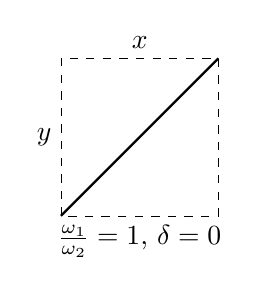
\begin{tikzpicture}
            \draw[domain=0:2*pi, smooth, samples=1000, thick] plot ({(sin(\x r)},{(sin(\x r))}) ;
            \draw [very thin, dashed] (-1,-1) -- node[left]{\(y\)} (-1,1) -- node[above]{\(x\)}
            (1,1) -- (1,-1) -- node[below]{\(\frac{\omega_1}{\omega_2}=1\), \(\delta=0\)} (-1,-1) ;
            \end{tikzpicture}
            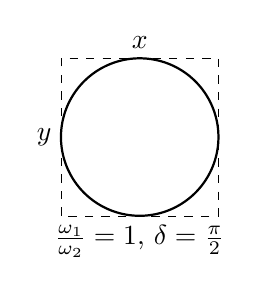
\begin{tikzpicture}
            \draw[domain=0:2*pi, smooth, samples=1000, thick] plot ({(sin(\x r)},{(cos(\x r))}) ;
            \draw [very thin, dashed] (-1,-1) -- node[left]{\(y\)} (-1,1) -- node[above]{\(x\)}
            (1,1) -- (1,-1) -- node[below]{\(\frac{\omega_1}{\omega_2}=1\),
            \(\delta=\frac{\pi}{2}\)} (-1,-1) ;
            \end{tikzpicture}
            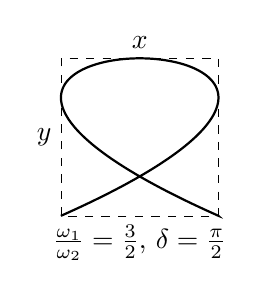
\begin{tikzpicture}
            \draw[domain=0:2*pi, smooth, samples=1000, thick] plot ({(sin(3*\x r)},{(cos(2*\x r)}) ;
            \draw [very thin, dashed] (-1,-1) -- node[left]{\(y\)} (-1,1) -- node[above]{\(x\)}
            (1,1) -- (1,-1) -- node[below]{\(\frac{\omega_1}{\omega_2}=\frac{3}{2}\),
            \(\delta=\frac{\pi}{2}\)} (-1,-1) ;
            \end{tikzpicture}
            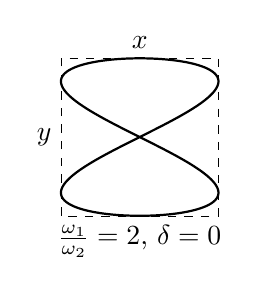
\begin{tikzpicture}
            \draw[domain=0:2*pi, smooth, samples=1000, thick] plot ({(sin(2*\x r)},{(sin(\x r))}) ;
            \draw [very thin, dashed] (-1,-1) -- node[left]{\(y\)} (-1,1) -- node[above]{\(x\)}
            (1,1) -- (1,-1) -- node[below]{\(\frac{\omega_1}{\omega_2}=2\), \(\delta=0\)} (-1,-1) ;
            \end{tikzpicture}
            
            
            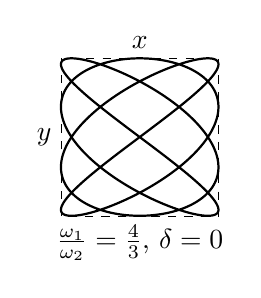
\begin{tikzpicture}
            \draw[domain=0:2*pi, smooth, samples=1000, thick] plot ({(sin(4*\x r)},{(sin(3*\x r))})
            ; \draw [very thin, dashed] (-1,-1) -- node[left]{\(y\)} (-1,1) -- node[above]{\(x\)}
            (1,1) -- (1,-1) -- node[below]{\(\frac{\omega_1}{\omega_2}=\frac{4}{3}\), \(\delta=0\)}
            (-1,-1) ;
            \end{tikzpicture}
            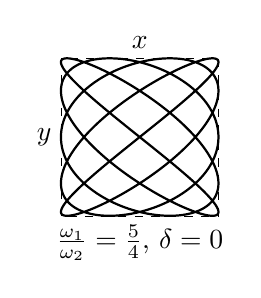
\begin{tikzpicture}
            \draw[domain=0:2*pi, smooth, samples=1000, thick] plot ({(sin(5*\x r)},{(sin(4*\x r))})
            ; \draw [very thin, dashed] (-1,-1) -- node[left]{\(y\)} (-1,1) -- node[above]{\(x\)}
            (1,1) -- (1,-1) -- node[below]{\(\frac{\omega_1}{\omega_2}=\frac{5}{4}\), \(\delta=0\)}
            (-1,-1) ;
            \end{tikzpicture}
            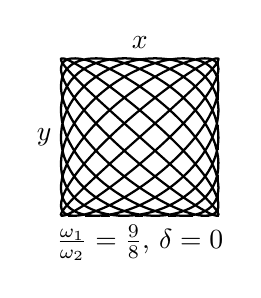
\begin{tikzpicture}
            \draw[domain=0:8*pi, smooth, samples=1000, thick] plot ({(sin(9*\x r)},{(sin(8*\x r ))})
            ; \draw [very thin, dashed] (-1,-1) -- node[left]{\(y\)} (-1,1) -- node[above]{\(x\)}
            (1,1) -- (1,-1) -- node[below]{\(\frac{\omega_1}{\omega_2}=\frac{9}{8}\), \(\delta=0\)}
            (-1,-1) ;
            \end{tikzpicture}
            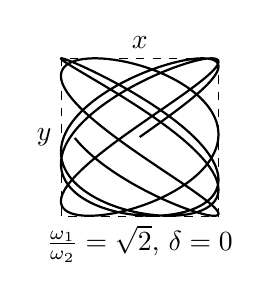
\begin{tikzpicture}
            \draw[domain=0:8*pi, smooth, samples=1000, thick] plot ({(sin(sqrt(2)*\x r)},{(sin(\x
            r))}) ; \draw [very thin, dashed] (-1,-1) -- node[left]{\(y\)} (-1,1) --
            node[above]{\(x\)} (1,1) -- (1,-1) --
            node[below]{\(\frac{\omega_1}{\omega_2}=\sqrt{2}\), \(\delta=0\)} (-1,-1) ;
            \end{tikzpicture}
            
            \caption{Wybrane krzywe Lissajous}
            \label{fig:lissajous1}
        \end{figure}
        Krzywe są zamknięte tylko wtedy, gdy stosunek \(\omega_1/\omega_2\) jest liczbą wymierną.
        Stosunek ten można wyznaczyć z rysunku korzystając z następującej metody: rysujemy dwie
        proste równoległe odpowiednio do osi \(x\) i \(y\) tak aby przecinały one krzywą w punktach
        różnych od przecięć krzywej ze sobą, a następnie zliczamy punkty przecięcia narysowanych
        prostych z krzywą Lissajous.
        
        \begin{figure}[ht]
            \centering
            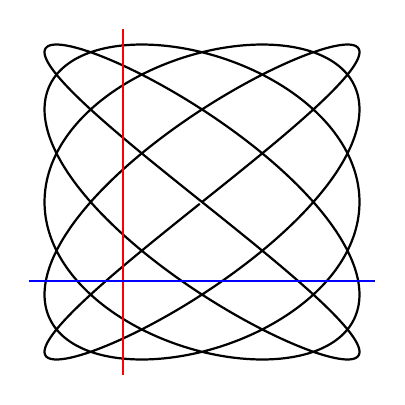
\begin{tikzpicture}
            \draw[domain=0:2*pi, smooth, samples=1000, thick] plot ({(2*sin(5*\x r)},{(2*sin(4*\x
            r))}) ; \draw[color=red, thick] (-1, 2.2) -- (-1,-2.2); \draw[color=blue, thick] (-2.2,
            -1) -- (2.2,-1);
            \end{tikzpicture}
            \caption{Metoda wyznaczania stosunku
            \(\omega_1/\omega_2=\textcolor{red}{n}/\textcolor{blue}{n}\) z rysunku}
            \label{fig:lissajous2}
        \end{figure}
        

        \subsection{Fale w ośrodkach sprężystych}
        \subsubsection{Jednowymiarowe równanie falowe}
        Fala (jednowymiarowa) to matematycznie rozwiązanie równania falowego
        \begin{equation*}
            \pdv[2]{f}{z}=\frac{1}{c^2}\pdv[2]{f}{t}\,,
        \end{equation*}
        gdzie \(f=f(z,t)\) jest funkcją opisującą kształt fali w danej chwili, a \(c\) jest
        prędkością rozchodzenia fali wzdłuż osi \(z\).\\
        Wyprowadzimy jednowymiarowe równanie falowe rozpatrując drgania poprzeczne naprężonej
        struny. Zakładamy, że wychylenia struny \(f(z,t)\) są niewielkie tak, że naprężenie \(T\)
        struny jest takie samo w każdym jej punkcie, a sama struna jest cały czas prawie równoległa
        do osi \(z\). Niech \(\mu\) oznacza gęstość liniową struny. Rozpatrzmy fragment struny o
        masie \(\mu\sqrt{\dd{f}^2+\dd{z}^2}\approx\mu \dd{z}\). Z II zasady dynamiki mamy
        \begin{equation*}
        \begin{split}
            F_z&=T\cos(\phi+\dd{\phi})-\cos\phi\approx 0\\
            F_y&=T\sin(\phi+\dd{\phi})-T\sin\phi\\
            &=T(\sin\phi\cos \dd{\phi}+\sin \dd{\phi}\cos \phi-\sin \phi)\approx T\cos\phi\,\dd{\phi}\approx T\dd{\phi}\,,
        \end{split}
        \end{equation*}
        oraz
        \begin{equation*}
            F_y=\mu\frac{\partial^2f}{\partial t^2}\dd{z}=T\frac{\partial \phi}{\partial z}\dd{z}\,.
        \end{equation*}
        Jednocześnie dla małych \(\phi\approx \tan\phi =\frac{\partial f}{\partial z}\), zatem
        \begin{equation*}
            \mu\frac{\partial^2f}{\partial t^2} =T\frac{\partial^2f}{\partial z^2}\,,
        \end{equation*}
       co, po podstawieniu \(c=\sqrt{T/\mu}\) daje dokładnie równanie falowe w jednym wymiarze.\\
       Udowodnimy teraz, że dowolne rozwiązanie powyższego równania falowego ma postać
       \begin{equation*}
           f(z,t)=\alpha(z-ct)+\beta(z+ct)\,,
       \end{equation*}
      gdzie \(\alpha\), \(\beta\) są pewnymi funkcjami. Zauważmy, że funkcja \(\alpha\) opisuje
      niezmieniający się w czasie kształt \(\alpha(z,0)=\alpha_0(z)\) poruszający się w stronę
      większych \(z\) z prędkością \(c\). Istotnie dla \(t=0\) kształt fali jest opisany funkcją
      \(\alpha(z)\), ale \(\alpha(z-c\cdot 0)=\alpha((z+ct)-ct)\), zatem widzimy, iż po czasie \(t\)
      punkt należący do fali o współrzędnych \((z,\alpha(z))\) przesunął się o odległość \(ct\) w
      prawo. Wprowadźmy zmienne
      \begin{equation*}
          \eta=z+ct\,,\quad \xi=z-ct\,.
      \end{equation*}
      Wówczas
      \begin{equation*}
      \begin{split}
          &\pdv{}{z}=\pdv{\eta}{z}\pdv{}{\eta}+\pdv{\xi}{z}\pdv{}{\xi}=\pdv{}{\eta}+\pdv{}{\xi}\\
          &\pdv{}{t}=\pdv{\eta}{t}\pdv{}{\eta}+\pdv{\xi}{t}\pdv{}{\xi}=c\pdv{}{\eta}-c\pdv{}{\xi}\,,
      \end{split}
      \end{equation*}
        zatem równanie falowe możemy przepisać do postaci
        \begin{equation*}
            c^2\left(\pdv[2]{f}{\eta}+\pdv[2]{f}{\xi}+2\pdv[2]{f}{\eta}{\xi}\right)=c^2\pdv[2]{f}{\eta}-2c^2\pdv[2]{f}{\eta}{\xi}+c^2\pdv[2]{f}{\xi}\,,
        \end{equation*}
        skąd otrzymujemy, iż w nowych zmiennych \((\eta,\xi)\) równanie falowe ma postać
        \begin{equation*}
            \pdv[2]{f}{\eta}{\xi}=0\,.
        \end{equation*}
        Oznaczmy \(\pdv{f}{\xi}=h(\eta,\xi)\), wówczas
        \begin{equation*}
            \pdv{h}{\eta}=0\,,
        \end{equation*}
        czyli \(h=h(\xi)\). Analogicznie, oznaczając \(\pdv{f}{\eta}=g(\eta,\xi)\), otrzymujemy
        \(g=g(\eta)\), skąd
        \begin{equation*}
            f(z,t)=\int h(\xi)\dd{\xi}+\int g(\eta)\dd{\eta}=\alpha(\xi)+\beta(\eta)=\alpha(z-ct)+\beta(z+ct)\,.
        \end{equation*}
        \subsubsection{Metoda separacji zmiennych}
        Podobnie jak inne równania różniczkowe cząstkowe, również równanie falowe można próbować
        rozwiązać \textit{metodą separacji zmiennych}. Istotnie sprawdźmy, czy istnieją rozwiązania
        równania falowego postaci
        \begin{equation*}
            f(z,t)=\Psi(z)\Phi(t)\,.
        \end{equation*}
        Podstawiając to wyrażenie do równania falowego otrzymujemy
        \begin{equation*}
            \Psi(z)\dv[2]{\Phi}{t}=c^2\Phi(t)\dv[2]{\Psi}{z}\,,
        \end{equation*}
        czyli
        \begin{equation*}
            \frac{1}{\Phi}\dv[2]{\Phi}{t}=\frac{c^2}{\Psi}\dv[2]{\Psi}{z}\,.
        \end{equation*}
        Zauważmy teraz, że lewa strona jest równa pewnej funkcji \(G(t)\), a prawa pewnej funkcji
        \(F(z)\). Aby powyższa równość zachodziła dla dowolnych \(z\), \(t\) musimy mieć
        \begin{equation*}
            \frac{1}{\Phi}\dv[2]{\Phi}{t}=\frac{c^2}{\Psi}\dv[2]{\Psi}{z}=-\omega^2\,,
        \end{equation*}
        gdzie \(\omega\) jest pewną stałą. Otrzymujemy zatem układ równań różniczkowych zwyczajnych
        \begin{equation*}
            \begin{split}
                &\dv[2]{\Phi}{t}+\omega^2\Phi=0\\
                &\dv[2]{\Psi}{z}+\frac{\omega^2}{c^2}\Psi=0
            \end{split}\quad\,.
        \end{equation*}
        Oznaczając \(k:=\omega/c\) otrzymujemy oczywiście
        \begin{equation*}
            \begin{split}
                &\Phi(t)=A\sin\omega t+B\cos\omega t\\
                &\Psi(z)=C\sin kz+D\cos kz
            \end{split}\quad\,.
        \end{equation*}
        Funkcja \(f(z,t)=\Phi(t)\Psi(z)\) spełnia zatem równanie falowe dla \(\Phi\), \(\Psi\)
        danych powyżej. Nie jest to jednak rozwiązanie ogólne. gdyż w ogólności nie spełnia warunków
        brzegowych (tj. zadania wartości funkcji dla określonych \(z_1\), \(z_2\), ...) ani warunków
        początkowych (tj. zadania kształtu \(f(z,0)=f_0(z)\) i początkowych prędkości
        \(\pdv{f}{t}\,(z,0)=\dot{f}_0(z)\)). Okazuje się jednak, iż dla konkretnych problemów
        powyższe rozwiązanie pozwala skonstruować rozwiązanie ogólne.
        \subsubsection{Fale tłumione}
        Zanim przejdziemy do rozwiązania zagadnienia fal w strunie o skończonej długości, podamy
        równanie falowe z liniowym członem tłumiącym. Istotnie zakładając, iż siła oporu działająca
        na strunę (np znajdującą się w lepkim  ośrodku) jest wprost proporcjonalna do \(\pdv{f}{t}\)
        otrzymujemy
        \begin{equation*}
            \pdv[2]{f}{t}+\frac{\gamma}{\mu}\pdv{f}{t}=c^2\pdv[2]{f}{z}\,,
        \end{equation*}
        gdzie \(\gamma\) jest współczynnikiem oporu i będziemy oznaczać \(2\beta:=\gamma/\mu\).
        \subsubsection{Rozwiązanie równania falowego dla struny o skończonej długości zamocowanej z obu stron}
        Jak łatwo sprawdzić metoda separacji zmiennych dla równania falowego z tłumieniem daje
        rozwiązanie (które będziemy oznaczać przez \(f_n(z,t)\))
        \begin{equation*}
            f_n(z,t)=(a_n\sin k_nz+b_n\cos k_nz)\e^{-\beta t}(A_n\sin\omega_n t+B_n\cos\omega_n t)\,,
        \end{equation*}
        gdzie \(\omega_n=\sqrt{k_n^2c^2-\beta^2}\). Dla struny o długości \(L\) zamocowanej z obu
        stron warunkiem brzegowym jest \(f(0,t)=f(L,t)=0\). Powyższa funkcja spełnia ten warunek,
        jeśli tylko \(b_n=0\) i \(k_n=\frac{n\pi}{L}\) (\(n\in\mathbb{Z}\)). Widzimy, zatem, że
        funkcja
        \begin{equation*}
            f_n(t)=\e^{-\beta t}\sin\left(\frac{n\pi z}{L}\right)(A_n\sin\omega_n t+B_n\cos\omega_n t)
        \end{equation*}
        spełnia równanie falowe i warunki brzegowe. Nie spełnia jednak w ogólności warunków
        początkowych. Zauważmy jednak, że ze względu na liniowość równania falowego również funkcja
        \begin{equation*}
            f(z,t)=\e^{-\beta t}\sum_{n=1}^\infty\sin\left(\frac{n\pi z}{L}\right)(A_n\sin\omega_n t+B_n\cos\omega_n t)
        \end{equation*}
        spełnia równanie falowe, przy jednoczesnym spełnieniu warunków brzegowych
        \(f(0,t)=f(L,t)=0\). Ta funkcja pozwala nam jednak spełnić warunki początkowe przy
        odpowiednim wyborze współczynników \(A_n\), \(B_n\). Istotnie dla \(t=0\)
        \begin{equation*}
            f(z,0)=f_0(z)=\sum_{n=1}^\infty B_n\sin\left(\frac{n\pi z}{L}\right)\,.
        \end{equation*}
        Dowolną sensowną funkcję \(f_0(z)\) określoną w \([0;L]\) można jednak przedstawić w tej
        postaci, na mocy twierdzenia Fouriera. Współczynniki \(B_n\) są dane wzorem
        \begin{equation*}
            B_n=\frac{2}{L}\int_0^Lf_0(z)\sin\left(\frac{n\pi z}{L}\right)\dd{z}\,.
        \end{equation*}
        Analogicznie mamy
        \begin{equation*}
            \dot{f}_0(z)=\sum_{n=1}^\infty (\omega_nA_n-\beta B_n)\sin\left(\frac{n\pi z}{L}\right)\,,
        \end{equation*}
        skąd
        \begin{equation*}
            A_n=B_n\frac{\beta}{\omega_n}+\frac{2}{\omega_nL}\int_0^L\dot{f}_0(z)\sin\left(\frac{n\pi z}{L}\right)\dd{z}\,,
        \end{equation*}
        gdzie
        \begin{equation*}
            \omega_n=\sqrt{\left(\frac{n\pi c}{L}\right)^2-\beta^2}\,.
        \end{equation*}
        Oczywiście zakładamy tutaj, iż \(\frac{\pi c}{L}>\beta\).
        \subsubsection{Przenoszenie energii}
        Fale mechaniczne przenoszą energię bez transportu energii. Moc fali sinusoidalnej można
        obliczyć korzystając ze wzoru \(P=F_y\frac{\partial y}{\partial t}\), skąd mamy
        \begin{equation*}
            P=T\frac{\partial \psi}{\partial x}\frac{\partial \psi}{\partial t}\,,
        \end{equation*}
        co dla fali sinusoidalnej \(\psi(x,t)=A\cos(kx-\omega t+\delta)\) daje
        \begin{equation*}
            P=-Tk\omega A^2\sin^2(kx-\omega t+\delta)=-\mu c\omega^2 A^2\sin^2(kx-\omega t+\delta)\,.
        \end{equation*}
        Wartość średnia z \(|P|\) wynosi
        \begin{equation*}
            \langle |P|\rangle =\frac{1}{2}\mu c\omega^2 A^2\,,
        \end{equation*}
        a natężenie fali \(I\)
        \begin{equation*}
            I=\frac{1}{2}\varrho c\omega^2A^2\,.
        \end{equation*}
        \subsubsection{Interferencja}
        Ponieważ rozwiązaniami równania falowego w postaci sinusoidalnej są funkcje \(\psi_{++}\),
        \(\psi_{--}\), \(\psi_{+-}\), \(\psi_{-+}\) i jest to równanie liniowe, więc również
        superpozycje tych funkcji są rozwiązaniami równania falowego. Dodając do siebie dowolne trzy
        z wymienionych funkcji dostajemy jedną z tych funkcji, nie jest to więc interesujący
        przypadek. Dodając do siebie wszystkie funkcje otrzymujemy \(\psi=0\) co również nie jest
        interesujące. Interesujące natomiast są sumy (przyjmujemy, że dla wszystkich funkcji \(A\),
        \(\delta\), \(\omega\) i \(k\) są takie same):
        \begin{equation*}
        \begin{split}
            &\psi_{++}+\psi_{+-}=2A\cos\left(kx+\delta\right)\cos\omega t\\
            &\psi_{++}+\psi_{-+}=2A\cos kx\cos\left(\omega t+\delta\right)\\
            &\psi_{--}+\psi_{+-}=2A\cos kx\cos(\omega t-\delta)\\
            &\psi_{--}+\psi_{-+}=2A\cos(kx-\delta)\cos\omega t
        \end{split}\,.
        \end{equation*}
        Zauważmy, że jeśli \(\delta=0\) to wszystkie te sumy dają wyrażenie \(2A\cos kx\cos\omega
        t\). Fale opisane tymi równaniami to tzw. \textit{fale stojące}. Ich cechą jest to, że się
        nie poruszają, tzn. są punkty \(x\) dla których \(y(t)=0\). Dla \(\delta=0\) te punkty
        wyznacza równanie \(\cos kx=0\), zatem są to punkty o współrzędnej \(x\) równej
        \(\lambda/4\), \(3\lambda/4\), ... . W strunie o długości \(L\) zamocowanej po obu stronach
        mogą zatem powstać fale stojące o długościach
        \begin{equation*}
            \lambda_n =\frac{2L}{n+1}\quad n=0,1,2,...\,.
        \end{equation*}
        W strunie (pręcie) zamocowanej tylko z jednej strony mogą powstać fale stojące o długościach
        \begin{equation*}
            \lambda_n=\frac{4L}{2n+1}\quad n=0,1,2,...\,.
        \end{equation*}
        \subsubsection{Dudnienia}
        Fale stojące są przykładem tzw. interferencji w przestrzeni, ale istnieje również
        interferencja w czasie. Rozpatrzmy złożenie drgań \(x_1(t)=A\sin\omega_1t\) i
        \(x_2(t)=A\sin\omega_2t\)
        \begin{equation*}
            x_1+x_2=2A\cos\left(\frac{\omega_1-\omega_2}{2}t\right)\sin\left(\frac{\omega_1+\omega_2}{2}t\right)=A(t)\sin\left(\frac{\omega_1+\omega_2}{2}t\right)\,.
        \end{equation*}
        Ponieważ \(I\propto A^2\), więc obliczmy \(A^2(t)\)
        \begin{equation*}
            A^2(t)=4A^2\cos^2\left(\frac{\omega_1-\omega_2}{2}t\right)=2A^2+2A^2\cos\{(\omega_1-\omega_2)t\}\,.
        \end{equation*}
        Częstość \(\omega_\text{mod}=\omega_1-\omega_2\) nazywamy częstością modulacji głośności
        (modulacji dudnień).
        
        \subsubsection{Efekt Dopplera}
        Zjawisko Dopplera polega na pozornej zmianie częstotliwości odbieranej fali na skutek
        wzajemnego ruchu obserwatora lub/i źródła. Częstotliwość \(f'\) odbierana przez obserwatora
        jest dana wzorem
        \begin{equation*}
            f'=f\left(\frac{c_\text{ef}+ v_o\cos\theta_o}{c_\text{ef}- v_z\cos\theta_z}\right)\,,
        \end{equation*}
        gdzie \(c_\text{ef}\) jest efektywną prędkością dźwięku (prędkością dźwięku modyfikowaną
        składową prędkości wiatru wzdłuż odcinka łączącego obserwatora ze źródłem)
        \begin{equation*}
            c_\text{ef}=c+\mathbf{v}_\text{wind}\cdot \mathbf{\hat r}_{zo}\,,
        \end{equation*}
        \(v_o\) jest szybkością obserwatora, \(v_z\) jest prędkością źródła, \(\theta_o\) jest kątem
        między wektorem prędkości obserwatora a odcinkiem łączącym obserwatora ze źródłem,
        \(\theta_z\) jest kątem między wektorem prędkości źródła a odcinkiem łączącym obserwatora ze
        źródłem.
        
\end{document}